%% Manuscript built on Elsevier's elsarticle template (numbered citation style).
%% Skeleton follows elsarticle-template-num.tex; the Methodology section is filled in.
%% Compile: pdflatex manuscript.tex (run twice for cross-references).

\documentclass[times, review, 10pt]{elsarticle}

%% The amssymb package provides various useful mathematical symbols
\usepackage{amssymb}
%% The amsmath package provides various useful equation environments.
\usepackage{amsmath}
%% The amsthm package provides extended theorem environments
\usepackage{amsthm}
%% Algorithm typesetting
\usepackage{algorithm}
\usepackage{algpseudocode}
%% Bold math symbols
\usepackage{bm}
%% Professional tables
\usepackage{booktabs}
%% Figures
\usepackage{graphicx}
%% Numbered contribution lists with custom (1) labels
\usepackage{enumerate}
%% Caption style aligned with the Pattern Recognition template: "Fig. 1." / "Table 1."
\usepackage{caption}
\captionsetup{labelsep=period}
\renewcommand{\figurename}{Fig.}

%% Lightweight theorem environments for the scatter-equivalence result.
\newtheorem{proposition}{Proposition}
\newtheorem{remark}{Remark}

%% Convenience macros.
\newcommand{\R}{\mathbb{R}}
\newcommand{\Sph}{\mathbb{S}}
\newcommand{\norm}[1]{\left\lVert #1 \right\rVert}
\newcommand{\inner}[2]{\left\langle #1,\, #2 \right\rangle}
\newcommand{\Xnorm}{\mathcal{X}_{\mathrm{n}}}
\newcommand{\Lcross}{\mathcal{L}_{\mathrm{con}}}
\newcommand{\Lscat}{\mathcal{L}_{\mathrm{scat}}}
\newcommand{\Ltot}{\mathcal{L}}
\newcommand{\hh}{\bm{h}}
\newcommand{\zz}{\bm{z}}
\newcommand{\xx}{\bm{x}}
\newcommand{\ww}{\bm{w}}
\newcommand{\WW}{\bm{W}}
\newcommand{\mmu}{\bm{\mu}}

\journal{Pattern Recognition}

\begin{document}

\begin{frontmatter}

%% Title, authors and addresses

\title{Scatter-Regularized Cross-Multi-Kernel Contrastive
Learning for One-Class Anomaly Detection}

%% use optional labels to link authors explicitly to addresses:
%% \author[label1,label2]{}
%% \affiliation[label1]{organization={},...}

\author{} %% Author name

%% Author affiliation
\affiliation{organization={},%Department and Organization
            addressline={},
            city={},
            postcode={},
            state={},
            country={}}

%% Abstract
\begin{abstract}

One-class anomaly detection has attracted extensive research due to 
its broad application in identifying unforeseeable deviations. The idea 
of contrastive learning is one of the widely used methods 
in modern outlier analysis. Nevertheless, these methods mainly use cross-view 
consistency to model normal data, so they cannot effectively guarantee the absolute 
intra-class compactness crucial for identifying outliers. Moreover, they typically 
map data into a single, fixed geometric space and cannot effectively capture complex 
similarity structures across multi-scale data. In this work, we propose a Scatter-regularized 
Cross-Multi-Kernel (SCMK) contrastive framework for one-class anomaly detection. First, 
a bank of multi-scale Gaussian kernels is constructed to inject multi-resolution geometric priors. 
Second, a cross-kernel InfoNCE 
objective is defined to treat the kernel index as a distinct view and align the representations. 
Then, a novel multi-kernel scatter regularizer is introduced to explicitly compact the normal 
class within every kernel-induced space. Based on this idea, two complementary signals—an 
angular detector (linear OC-SVM) and a radial detector (RBF OC-SVM)—are fused via a per-sample 
maximum to quantify the anomaly scores. Finally, experimental comparisons with state-of-the-art 
methods on 20 benchmark datasets show that the proposed method has a significant improvement, 
achieving the highest mean AUC, and applies robustly to diverse dataset topologies.
\end{abstract}

%%Graphical abstract
\begin{graphicalabstract}
%\includegraphics{grabs}
\end{graphicalabstract}

%%Research highlights
\begin{highlights}
\item A cross-multi-kernel contrastive encoder reconciles multi-scale kernel
views by treating the kernel index as the contrastive view.
\item A multi-kernel scatter regularizer is proved equal to the average
within-class scatter and to one-class centroid multiple-kernel $k$-means.
\item A dual-signal detector fuses an angular (linear OC-SVM) and a radial (RBF
OC-SVM) score, staying robust across datasets where either single signal
collapses.
\end{highlights}

%% Keywords
\begin{keyword}
anomaly detection \sep multiple kernel learning \sep contrastive learning
\sep one-class classification \sep representation learning
\end{keyword}

\end{frontmatter}

%% main text

%% ======================================================================
\section{Introduction}
\label{sec:intro}

Anomaly detection---the task of identifying observations that deviate markedly
from the prevailing pattern of the data---underpins a broad range of
applications, including financial fraud detection, industrial fault diagnosis,
network-intrusion monitoring, and medical screening~\cite{pang2021review,
ruff2021unifying}. The defining difficulty of the problem is statistical:
anomalies are rare, heterogeneous, and largely unforeseeable, so the abnormal
class can be neither sampled exhaustively nor characterised in advance. This
rules out a conventional supervised formulation and motivates the
\emph{one-class} (semi-supervised) paradigm, in which a model is trained on
normal data alone and flags as anomalous any test instance that departs from the
learned notion of normality~\cite{scholkopf2001ocsvm,tax2004svdd}.

Classical one-class detectors realise this idea in a \emph{single, fixed}
similarity space. The one-class support vector machine
(OC-SVM)~\cite{scholkopf2001ocsvm} and support vector data description
(SVDD)~\cite{tax2004svdd} separate the normal data from the origin, or enclose
them in a minimal sphere, within one reproducing-kernel Hilbert space; density-
and distance-based methods such as LOF~\cite{breunig2000lof} and isolation
forests~\cite{liu2008iforest} likewise commit to one geometric prior. Their
accuracy therefore hinges critically on the choice of kernel and bandwidth, a
choice that does not transfer well across datasets and degrades in
high-dimensional, heterogeneous feature spaces. Deep one-class models alleviate
the fixed-geometry issue by \emph{learning} a representation: autoencoder-based
detectors~\cite{zhou2017rda} score samples by reconstruction error, while Deep
SVDD~\cite{ruff2018svdd} maps normal data into a compact hypersphere. Yet
reconstruction objectives are not inherently discriminative, hypersphere
objectives are prone to representational collapse, and---crucially---each of
these methods still summarises similarity through a \emph{single} learned
geometry.

Multiple kernel learning (MKL) offers a principled remedy to the single-geometry
limitation by combining a bank of kernels that encode complementary notions of
similarity at different scales~\cite{gonen2011mkl,lanckriet2004sdp}. Fusing such
views improves robustness and removes the burden of selecting one ``correct''
kernel, and the idea extends naturally to clustering through multiple-kernel
$k$-means and its centroid variants~\cite{liu2016mkkm,huang2012mkkm}. However,
classical MKL and MKKM are \emph{shallow}: they operate directly on the raw input
features and merely learn a set of scalar kernel weights, without inducing a
representation that a downstream detector can exploit. The expressive power of
modern representation learning is thus left untapped.

Contrastive representation learning provides exactly such expressive power. By
pulling together different ``views'' of the same instance and pushing apart views
of different instances, objectives such as InfoNCE~\cite{oord2018infonce} and
SimCLR~\cite{chen2020simclr} learn embeddings that transfer remarkably well, and
they have recently been adapted to anomaly detection~\cite{tack2020csi,
qiu2021neutral}. This suggests a natural marriage with MKL: treat the
\emph{kernel index itself as a contrastive view}, so that the embeddings produced
by different kernels for the same sample are aligned, while embeddings of
different samples remain separable. Such a cross-kernel contrastive encoder
reconciles multi-scale similarity within a learned representation. Nevertheless,
a subtle but consequential gap remains. The InfoNCE objective enforces only
\emph{cross-view consistency} (alignment of a sample's kernel views) and
\emph{instance discriminability} (uniformity over the sphere); it does not make
the normal class \emph{absolutely compact}. Indeed, the loss is invariant to
configurations that scatter normal embeddings widely across the representation
space as long as each sample's views agree. For one-class detection, however,
the compactness of the normal region is precisely the property that a downstream
detector relies upon. We identify this mismatch---\emph{consistency is not
compactness}---as the central obstacle to coupling contrastive learning with
one-class detection.

We resolve it with \emph{scatter-regularized cross-multi-kernel} contrastive
learning (SCMK). On top of a cross-kernel contrastive encoder built over a
multi-scale Gaussian kernel bank, we introduce a \emph{multi-kernel scatter
regularizer} that explicitly compacts the normal class within every
kernel-induced embedding space. The regularizer is derived from the one-class
specialisation of centroid multiple-kernel $k$-means, and we prove that it equals
---up to an additive constant---the average within-class scatter of the
unit-norm embeddings, thereby giving the heuristic a firm theoretical footing.
Combined with the uniformity pressure of the contrastive term, the scatter
penalty tightens the normal class without inducing collapse, yielding a
representation on which a simple and efficient \emph{linear} one-class SVM
suffices to score anomalies.

The main contributions of this work are summarised as follows.
\begin{enumerate}[\indent(1)]
\item We propose a cross-multi-kernel contrastive framework that treats the
kernel index as the contrastive view and aligns the embeddings of a multi-scale
kernel bank whose bandwidths are auto-calibrated by a median-distance heuristic
on the normal data.
\item We introduce a multi-kernel scatter regularizer and \emph{prove} that it is
equivalent to the average within-class scatter and to the one-class instance of
centroid multiple-kernel $k$-means, bridging multiple-kernel clustering theory
and contrastive anomaly detection.
\item We provide a collapse-avoidance analysis through the
alignment--uniformity lens, showing how the contrastive and scatter terms
balance, and we exploit the resulting representation with a lightweight
dual-signal detector that fuses an angular (linear OC-SVM) and a radial (RBF
OC-SVM) score, recovering the discriminative information that $\ell_2$
normalization alone discards.
\item Extensive experiments on twenty benchmark datasets against seven recent
detectors demonstrate that the proposed method attains the highest mean and most
stable detection accuracy among competitive baselines, and ablation studies isolate the
contribution of each component.
\end{enumerate}

The remainder of this paper is organized as follows.
Section~\ref{sec:related} reviews related work on one-class anomaly detection,
multiple kernel learning and contrastive representation learning.
Section~\ref{sec:method} presents the proposed SCMK method.
Section~\ref{sec:exp} reports the experimental comparison, statistical tests,
runtime, parameter sensitivity and ablation studies.
Section~\ref{sec:conclusion} concludes the paper and outlines future work.

%% ======================================================================
\section{Related work}
\label{sec:related}

\subsection{One-class and deep anomaly detection}
\label{subsec:rel-ad}
Unsupervised anomaly detection has been studied for decades under a variety of
paradigms. Traditional approaches can be broadly grouped into statistical,
distance-based, density-based and clustering-based methods. Statistical methods
fit a model to the bulk of the data and flag observations that deviate
significantly from the assumed distribution~\cite{chandola2009survey}.
Distance-based methods treat points that lie far from most others in the feature
space as anomalous~\cite{knorr2000distance}, whereas density-based methods---of
which the Local Outlier Factor (LOF)~\cite{breunig2000lof} is the canonical
example---compare the local density of a point with that of its neighbours to
expose local outliers. Clustering- and partition-based methods instead group the
data and regard samples that fall far from any cluster, or that are easily
isolated as in the isolation forest~\cite{liu2008iforest}, as anomalies. Although effective on low-dimensional data, these
methods rest on explicit assumptions about the geometry of the normal
class---a roughly uniform distribution for distance-based methods, a
well-calibrated neighbourhood for density-based methods, or a fixed similarity
measure---and consequently degrade on high-dimensional, heterogeneous or
categorical data whose structure violates those assumptions.

A particularly influential family formalises detection as \emph{one-class}
classification: only normal data are available, and the task is to characterise
the compact region they occupy so that deviations can be flagged at test time.
The two canonical kernel-based formulations are the One-Class Support Vector
Machine (OC-SVM)~\cite{scholkopf2001ocsvm}, which separates the normal data from
the origin by a maximum-margin hyperplane in a reproducing-kernel Hilbert space,
and Support Vector Data Description (SVDD)~\cite{tax2004svdd}, which encloses the
normal data within a minimum-volume hypersphere; the two objectives coincide for
translation-invariant kernels. These shallow one-class detectors are effective
but remain sensitive to the choice of kernel and similarity measure and scale
poorly with dimension, which motivates coupling the one-class objective with a
learned representation.

Deep anomaly detection learns the representation jointly with the detector.
Autoencoder and robust-autoencoder approaches~\cite{zhou2017rda} flag samples with
large reconstruction error, and Deep SVDD~\cite{ruff2018svdd} learns a network that
maps normal data into a minimum-volume hypersphere, at the risk of trivial
collapse. A complementary line is self-supervised: geometric-transformation
prediction~\cite{golan2018geo} and its generalisation to non-image data,
GOAD~\cite{bergman2020goad}, detect anomalies through the predictability of
applied transformations.

\subsection{Multiple kernel learning}
\label{subsec:rel-mkl}
Multiple kernel learning combines several base kernels into a single, more
expressive kernel, typically by learning a convex combination of weights.
Foundational formulations cast weight learning as semidefinite or
gradient-based optimisation~\cite{lanckriet2004sdp,rakotomamonjy2008simplemkl},
and localised variants allow the combination to vary across the input
space~\cite{gonen2008localized}; see~\cite{gonen2011mkl} for a survey. In the
unsupervised setting, multiple-kernel $k$-means and its centroid (CMKKM) and
matrix-regularised variants~\cite{liu2016mkkm,huang2012mkkm} jointly optimise
cluster assignments and kernel weights, with diversity-promoting regularisers
discouraging redundant kernels. These techniques are, however, shallow---they act
on raw features and output only kernel weights. Our work retains the
multiple-kernel principle but lifts it into a learned embedding space, and it
repurposes the one-class CMKKM objective as a differentiable scatter
regularizer for representation learning rather than as a clustering criterion.

\subsection{Contrastive representation learning}
\label{subsec:rel-cl}
Contrastive learning has become a dominant paradigm for self-supervised
representation learning. InfoNCE~\cite{oord2018infonce} and
SimCLR~\cite{chen2020simclr} maximise agreement between augmented views of an
instance against a set of negatives, MoCo~\cite{he2020moco} maintains a momentum
queue of negatives, and BYOL~\cite{grill2020byol} and
SimSiam~\cite{chen2021simsiam} dispense with explicit negatives altogether. Wang
and Isola~\cite{wang2020uniformity} characterise the resulting geometry through
two competing properties, {alignment} of positive pairs and
{uniformity} of the embedding distribution on the hypersphere, an analysis
we invoke to explain why our scatter regularizer does not collapse the
representation. Whereas these methods generate views by stochastic data
augmentation, we obtain views from kernel diversity, and we observe that the
consistency enforced by contrastive learning does not by itself yield the
intra-class compactness required for one-class detection---a gap that our scatter
regularizer is designed to close.

\subsection{Positioning of this work}
\label{subsec:rel-pos}
SCMK sits at the intersection of the three threads above. From anomaly detection
it inherits the one-class formulation and an OC-SVM head; from multiple kernel
learning it inherits a multi-scale kernel bank and the centroid-MKKM compactness
principle; and from contrastive learning it inherits a representation objective,
which we adapt by treating the kernel index as the view. To our knowledge, the
combination of {kernel-as-view} contrastive learning with a scatter
regularizer that provably realises one-class CMKKM has not been explored, and it
is this combination that delivers a compact, kernel-fused representation amenable
to efficient linear one-class detection.

%% ======================================================================
\section{The proposed SCMK method}
\label{sec:method}

\subsection{Problem formulation and notation}
\label{subsec:problem}

Let
$\mathcal{X}=\{\xx_i\}_{i=1}^{N}$ with $\xx_i\in\R^{D}$ denote the data after
preprocessing,\footnote{Nominal attributes are one-hot encoded and numerical
attributes are min--max scaled to $[0,1]$, so that all feature dimensions share
a comparable range.} and let $y_i\in\{0,1\}$ be the latent label, where $y_i=0$
marks a normal instance and $y_i=1$ an anomaly. Only the normal subset
$\Xnorm=\{\xx_i : y_i=0\}$, of size $N_{\mathrm{n}}=|\Xnorm|$, is available at
training time; anomalies are neither observed nor simulated. The goal is to
learn a scoring function $a:\R^{D}\!\to\!\R$ such that $a(\xx)$ is large for
anomalies and small for normal points.

Our framework, termed \emph{scatter-regularized cross-multi-kernel}
contrastive learning (SCMK), couples a multiple-kernel contrastive encoder
with a one-class detection head. It comprises four components, summarised in
Algorithm~\ref{alg:scmk}:
(i) a multi-scale kernel bank that injects geometric priors at several
resolutions (Section~\ref{subsec:kernels});
(ii) a cross-kernel contrastive objective that aligns the views produced by
different kernels (Section~\ref{subsec:contrastive});
(iii) a multi-kernel scatter regularizer that explicitly compacts the normal
class in every kernel-induced embedding (Section~\ref{subsec:scatter}); and
(iv) a dual-signal one-class detector that fuses an angular and a radial OC-SVM
score to flag anomalies (Section~\ref{subsec:detection}).

\subsection{Multi-scale kernel bank}
\label{subsec:kernels}

To endow the encoder with multi-resolution sensitivity, we instantiate a bank
of $K$ Gaussian kernels whose bandwidths are anchored to the intrinsic scale of
the normal data. Let
\begin{equation}
\mathrm{med}
=\operatorname{median}\!\big\{\norm{\xx_i-\xx_j}_2 :
\xx_i,\xx_j\in\Xnorm,\ i\neq j\big\}
\label{eq:median}
\end{equation}
be the median pairwise Euclidean distance estimated \emph{from normal samples
only}, which prevents contamination of the scale statistic by outliers. The
$k$-th kernel is
\begin{equation}
\kappa_k(\bm{a},\bm{b})
=\exp\!\left(-\frac{\norm{\bm{a}-\bm{b}}_2^{2}}{2\,t_k^{2}}\right),
\qquad
t_k = r_k\cdot\mathrm{med},
\label{eq:gaussian}
\end{equation}
with multiplicative ratios $\{r_k\}_{k=1}^{K}=\{0.1,0.5,1.0,2.0,5.0\}$
($K=5$). Small ratios produce sharp kernels that resolve fine-grained local
neighbourhoods, whereas large ratios produce broad kernels that capture the
global manifold geometry. The bank therefore provides $K$ complementary
similarity measures that the contrastive stage will reconcile.

\subsection{Cross-kernel contrastive representation learning}
\label{subsec:contrastive}

\paragraph{Per-kernel embeddings.}
For each kernel we attach an independent, bias-free linear projection head
$g_k(\xx)=\WW_k\xx$ with $\WW_k\in\R^{d\times D}$, followed by
$\ell_2$ normalization,
\begin{equation}
\hh_{k,i}
=\frac{\WW_k\xx_i}{\norm{\WW_k\xx_i}_2}\in\Sph^{d-1},
\qquad k=1,\dots,K,
\label{eq:embedding}
\end{equation}
so that every embedding lives on the unit hypersphere $\Sph^{d-1}$. Removing the
bias keeps the representation centred at the origin, which is consistent with
the origin-separating hyperplane assumption of the downstream OC-SVM, while the
normalization equalises the scale across kernels.

\paragraph{Cross-kernel positive pairs.}
Whereas conventional contrastive learning forms positive pairs through
stochastic data augmentation, we treat the \emph{kernel index as the view}: the
two embeddings $\hh_{k,i}$ and $\hh_{l,i}$ of the \emph{same} sample under
\emph{different} kernels constitute a positive pair, and embeddings of distinct
samples are negatives. Consider a mini-batch of $B$ normal samples and a kernel
pair $(k,l)$. Stacking the two views yields
$\bm{F}^{(kl)}=[\hh_{k,1},\dots,\hh_{k,B},\hh_{l,1},\dots,\hh_{l,B}]^{\!\top}
\in\R^{2B\times d}$,
whose rows are indexed by $m,n\in\{1,\dots,2B\}$. The pairwise affinity is the
\emph{symmetrised kernel response} evaluated on the embeddings,
\begin{equation}
s^{(kl)}_{mn}
=\tfrac{1}{2}\big[\kappa_k(\bm{f}_m,\bm{f}_n)
+\kappa_l(\bm{f}_m,\bm{f}_n)\big].
\label{eq:affinity}
\end{equation}
Because the embeddings are unit-norm, the Gaussian response reduces to a
monotone function of cosine similarity,
$\kappa_k(\bm{f}_m,\bm{f}_n)
=\exp\!\big(-(1-\inner{\bm{f}_m}{\bm{f}_n})/t_k^{2}\big)$,
so $t_k^{2}$ plays the role of a contrastive temperature that is automatically
adapted to the data scale through Eq.~\eqref{eq:median}.

\paragraph{Cross-kernel InfoNCE.}
For anchor $n$, let $\pi(n)$ index its cross-view positive (i.e.\ $\pi(n)=n+B$
for $n\le B$ and $\pi(n)=n-B$ otherwise). The InfoNCE loss for the pair $(k,l)$
is
\begin{equation}
\Lcross^{(kl)}
=-\frac{1}{2B}\sum_{n=1}^{2B}
\log\frac{\exp\!\big(s^{(kl)}_{n,\pi(n)}\big)}
{\displaystyle\sum_{m\neq n}\exp\!\big(s^{(kl)}_{nm}\big)},
\label{eq:infonce}
\end{equation}
where the denominator excludes the self-similarity term $m=n$. Averaging over
all $\binom{K}{2}$ unordered kernel pairs gives the cross-kernel contrastive
objective
\begin{equation}
\Lcross
=\frac{1}{\binom{K}{2}}
\sum_{1\le k<l\le K}\Lcross^{(kl)}.
\label{eq:lcross}
\end{equation}
Minimising Eq.~\eqref{eq:lcross} drives the encoder to a \emph{view-invariant}
representation in which all kernels agree on the embedding of each normal
sample, i.e.\ $\hh_{k,i}\!\approx\!\hh_{l,i}$, while keeping distinct samples
mutually discriminable through the negative terms.

\subsection{Multi-kernel scatter regularization}
\label{subsec:scatter}

\paragraph{Motivation.}
The contrastive objective~\eqref{eq:lcross} enforces \emph{cross-kernel
consistency} but does not constrain the \emph{absolute compactness} of the
normal class: it is invariant to a rotation that spreads normal embeddings
across the sphere as long as the per-sample views remain aligned. A one-class
detector, however, benefits directly from a tightly concentrated normal region.
We therefore introduce a regularizer that minimises the dispersion of the normal
class within every kernel-induced embedding space, drawing on the one-class
specialisation of centroid multiple-kernel $k$-means (CMKKM).

\paragraph{Definition.}
Let $\mmu_k=\frac{1}{B}\sum_{i=1}^{B}\hh_{k,i}$ be the empirical centroid of the
normal embeddings under kernel $k$. The multi-kernel scatter penalty is
\begin{equation}
\Lscat
=-\frac{1}{K}\sum_{k=1}^{K}\norm{\mmu_k}_2^{2}.
\label{eq:lscat}
\end{equation}
It is computed in $O(KBd)$ time --- a single mean per kernel --- and thus adds
negligible overhead.

\paragraph{Exact equivalence to within-class scatter.}
The next result shows that Eq.~\eqref{eq:lscat} is not a heuristic surrogate but
is \emph{exactly} (up to an additive constant) the average within-class scatter
of the normal embeddings.

\begin{proposition}[Scatter equivalence]
\label{prop:scatter}
For unit-norm embeddings $\hh_{k,i}\in\Sph^{d-1}$, define the average normalised
within-class scatter
$\sigma^2=\frac{1}{NK}\sum_{k=1}^{K}\sum_{i=1}^{N}\norm{\hh_{k,i}-\mmu_k}_2^{2}$.
Then
\begin{equation}
\sigma^2 = 1 + \Lscat .
\label{eq:equiv}
\end{equation}
Consequently, minimising $\Lscat$ is equivalent to minimising the within-class
scatter $\sigma^2$, and equivalently to maximising the mean intra-class kernel
alignment $\frac{1}{NK}\sum_k\sum_{i,j}\inner{\hh_{k,i}}{\hh_{k,j}}
=\frac{1}{K}\sum_k\norm{\mmu_k}_2^2$.
\end{proposition}

\begin{proof}
Fix a kernel $k$. Expanding the squared norm and using $\norm{\hh_{k,i}}_2^2=1$,
\begin{align}
\sum_{i=1}^{N}\norm{\hh_{k,i}-\mmu_k}_2^{2}
&=\sum_{i=1}^{N}\!\Big(\norm{\hh_{k,i}}_2^{2}
-2\inner{\hh_{k,i}}{\mmu_k}+\norm{\mmu_k}_2^{2}\Big)\nonumber\\
&=N-2N\norm{\mmu_k}_2^{2}+N\norm{\mmu_k}_2^{2}
=N\big(1-\norm{\mmu_k}_2^{2}\big),
\label{eq:proofstep}
\end{align}
where $\sum_i\inner{\hh_{k,i}}{\mmu_k}=N\inner{\mmu_k}{\mmu_k}=N\norm{\mmu_k}_2^2$
follows from the definition of $\mmu_k$. Averaging Eq.~\eqref{eq:proofstep} over
$k$ and dividing by $N$ yields
$\sigma^2=1-\frac{1}{K}\sum_k\norm{\mmu_k}_2^2=1+\Lscat$. The
alignment identity is immediate from
$\sum_{i,j}\inner{\hh_{k,i}}{\hh_{k,j}}=N^2\norm{\mmu_k}_2^2$.
\end{proof}

\begin{remark}[Connection to one-class CMKKM]
The one-class instance of centroid multiple-kernel $k$-means maximises
$\operatorname{Tr}(\bm{H}^{\!\top}\bm{K}_{\eta}\bm{H})$ with a single soft cluster
indicator $\bm{H}=N^{-1/2}\bm{1}$ and a convex kernel combination
$\bm{K}_{\eta}=\sum_k\eta_k\,\Phi_k\Phi_k^{\!\top}$, where
$\Phi_k=[\hh_{k,1},\dots,\hh_{k,N}]^{\!\top}$ realises a linear kernel on the
embeddings. A short calculation gives
$\operatorname{Tr}(\bm{H}^{\!\top}\bm{K}_{\eta}\bm{H})
=N\sum_k\eta_k\norm{\mmu_k}_2^2$, which under uniform weights
$\eta_k=1/K$ equals $-N\,\Lscat$. Hence $\Lscat$ is precisely the
(negated, scale-normalised) one-class CMKKM compactness objective, providing a
multiple-kernel-learning justification for the penalty.
\end{remark}

\subsection{Joint objective and collapse avoidance}
\label{subsec:joint}

The encoder $\{\WW_k\}_{k=1}^{K}$ is trained by minimising the combined loss
\begin{equation}
\Ltot=\Lcross+\lambda\,\Lscat,
\label{eq:total}
\end{equation}
where $\lambda\ge 0$ trades off cross-kernel consistency against intra-class
compactness; $\lambda=0$ recovers the purely contrastive backbone.

A natural concern is representational \emph{collapse}: the scatter term alone is
trivially minimised ($\Lscat=-1$) when all embeddings of a kernel coincide
($\norm{\mmu_k}_2=1$). This degenerate solution is, however, suppressed by the
contrastive term. In the alignment--uniformity decomposition of contrastive
learning, the numerator of Eq.~\eqref{eq:infonce} promotes \emph{alignment} of
positives while the log-sum-exp denominator promotes \emph{uniformity} of the
embedding distribution on the sphere, which is maximised only by a spread-out
configuration and is therefore directly opposed to collapse. The joint
objective~\eqref{eq:total} thus realises a controlled balance: $\Lscat$ pulls
each normal class towards its centroid, $\Lcross$ prevents the normal embeddings
from degenerating to a point and keeps different samples separable, and
$\lambda$ governs the equilibrium. The unit-sphere constraint additionally
bounds $\norm{\mmu_k}_2\le 1$, so the penalty cannot diverge.

\subsection{Dual-signal anomaly scoring}
\label{subsec:detection}

After training, the projection heads are frozen and each sample $\xx_i$ is
described by \emph{two complementary signals} read off the raw projections
$\WW_k\xx_i$: the \emph{angular} position of its unit-norm embeddings and the
\emph{radial} magnitude of those projections. These signals carry
non-redundant discriminative information, and which of them separates the
normal and anomalous classes is dataset-dependent. We therefore build a
detector for each and fuse their scores.

\paragraph{Directional signal: linear OC-SVM on the angular embedding.}
The unit-norm embeddings $\hh_{k,i}$ retain only the angular position of a
sample on each kernel sphere---exactly the geometry that the scatter
regularizer~\eqref{eq:lscat} compacts. Concatenating the $K$ views,
\begin{equation}
\zz_i=\big[\hh_{1,i}^{\!\top},\hh_{2,i}^{\!\top},\dots,
\hh_{K,i}^{\!\top}\big]^{\!\top}\in\R^{Kd},
\label{eq:concat}
\end{equation}
fuses them into a single descriptor, and a linear-kernel OC-SVM fitted on the
normal embeddings $\{\zz_i : y_i=0\}$ by solving
\begin{equation}
\min_{\ww,\rho,\bm{\xi}}\ \
\tfrac{1}{2}\norm{\ww}_2^{2}-\rho
+\frac{1}{\nu N_{\mathrm{n}}}\sum_{i:\,y_i=0}\xi_i
\quad\text{s.t.}\quad
\inner{\ww}{\zz_i}\ge\rho-\xi_i,\ \ \xi_i\ge 0,
\label{eq:ocsvm}
\end{equation}
yields the \emph{directional score}
$s^{\mathrm{dir}}_i=\rho-\inner{\ww}{\zz_i}$, where $\nu\in(0,1]$ upper-bounds
the fraction of normal training points allowed outside the decision region. A
linear separator suffices here because the contrastive and scatter objectives
jointly mould the normal class into a compact, nearly linearly separable cone
on the product of spheres $(\Sph^{d-1})^{K}$; this score is informative
whenever the normal/anomaly contrast is \emph{angular}.

\paragraph{Magnitude signal: RBF OC-SVM on the projection norms.}
The $\ell_2$ normalization in Eq.~\eqref{eq:embedding} deliberately discards the
projection norms $r_{k,i}=\norm{\WW_k\xx_i}_2$. Yet these norms are themselves
discriminative: trained on normal data alone, each head maps normal samples into
a characteristic energy band, whereas anomalies---lying off the learned
manifold---are projected to markedly different, typically larger, norms. We
collect the per-kernel norms into a magnitude vector
\begin{equation}
\bm{r}_i=\big[r_{1,i},r_{2,i},\dots,r_{K,i}\big]^{\!\top}\in\R^{K},
\label{eq:rmag}
\end{equation}
and fit an \emph{RBF}-kernel OC-SVM on the normal norms $\{\bm{r}_i : y_i=0\}$,
producing the \emph{magnitude score} $s^{\mathrm{mag}}_i$. The RBF kernel is
essential: a \emph{linear} OC-SVM on norms admits a sign-reversed optimum---when
the normal norms are small, the separating direction turns negative and labels
large-norm anomalies as inliers---whereas the RBF density model, centred on the
compact small-norm normal cluster, correctly assigns high scores to the
large-norm outliers lying outside it. This score is informative whenever the
contrast is \emph{radial}.

\paragraph{Score fusion.}
On a given dataset one signal may be essentially uninformative---most strikingly,
the directional score collapses to near-chance when normal and anomalous samples
are angularly indistinguishable but differ in projection energy. Without assuming
\emph{a priori} which regime holds, we fuse the two detectors by a per-sample
maximum of min--max-normalised scores,
\begin{equation}
a(\xx_i)=\max\!\Big(\widetilde{s}^{\mathrm{dir}}_i,\ \widetilde{s}^{\mathrm{mag}}_i\Big),
\qquad
\widetilde{s}^{\,\bullet}_i=
\frac{s^{\bullet}_i-\min_j s^{\bullet}_j}{\max_j s^{\bullet}_j-\min_j s^{\bullet}_j},
\label{eq:fuse}
\end{equation}
so that a sample flagged by \emph{either} detector receives a high anomaly
score. The fusion needs no prior knowledge of which signal is informative and,
as the ablation in Section~\ref{subsec:exp-ablation} confirms, remains robust on
datasets where either single signal collapses while never trailing the stronger
signal by a meaningful margin. Fig.~\ref{fig:sphere} makes this complementarity
geometric: on a direction-dominant dataset the anomalies stay on the sphere but
cluster to one angular region, whereas on a magnitude-dominant dataset they are
angularly mixed with the normal class yet bulge far outside the sphere---so a
single detector necessarily fails on one regime, while the max-fusion captures
both.

\begin{figure}[t]
\centering
\begin{minipage}{0.49\linewidth}\centering
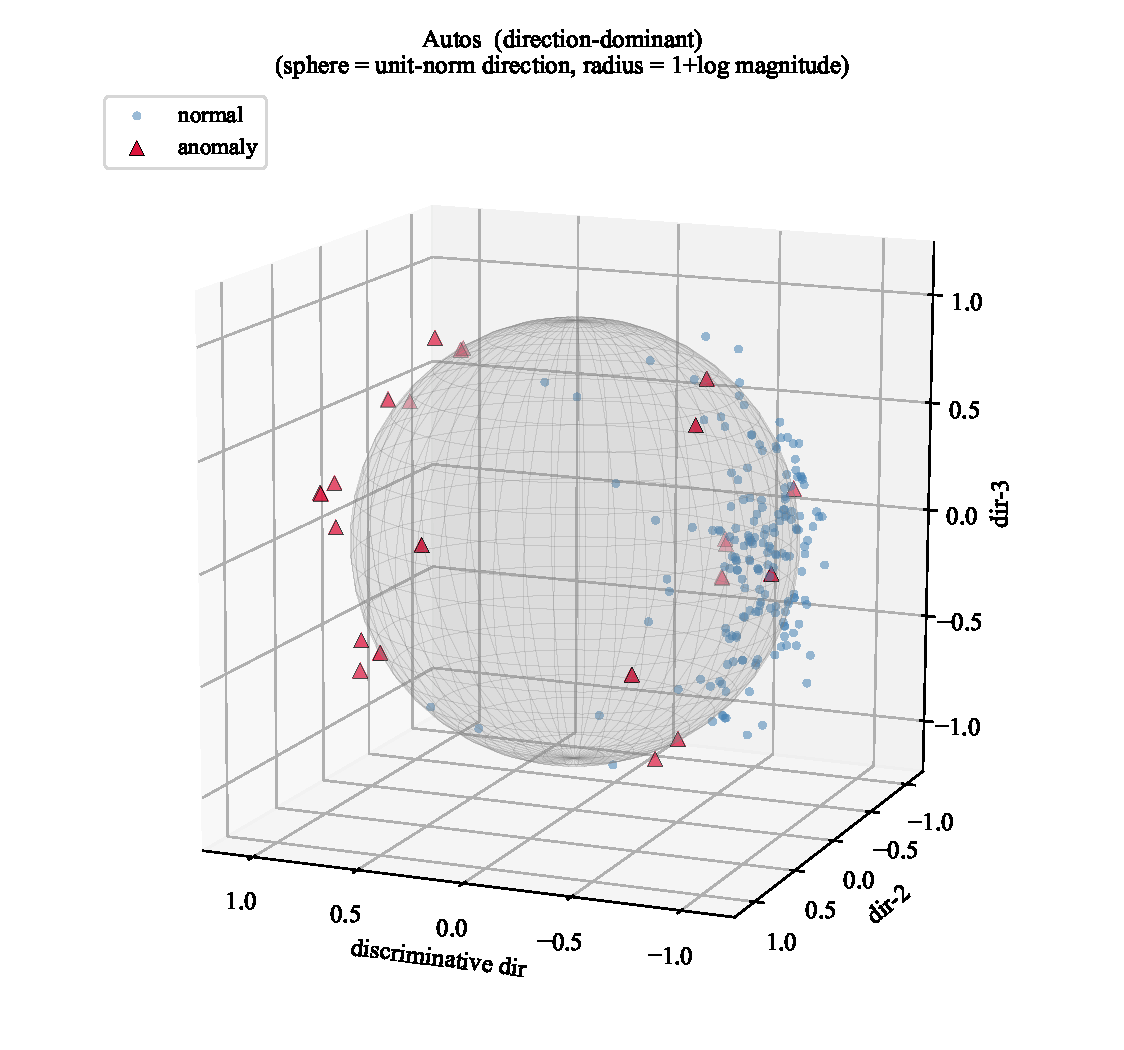
\includegraphics[width=\linewidth]{fig_sphere_autos.pdf}\\[-2pt]
{\small (a) Autos --- direction-dominant}
\end{minipage}\hfill
\begin{minipage}{0.49\linewidth}\centering
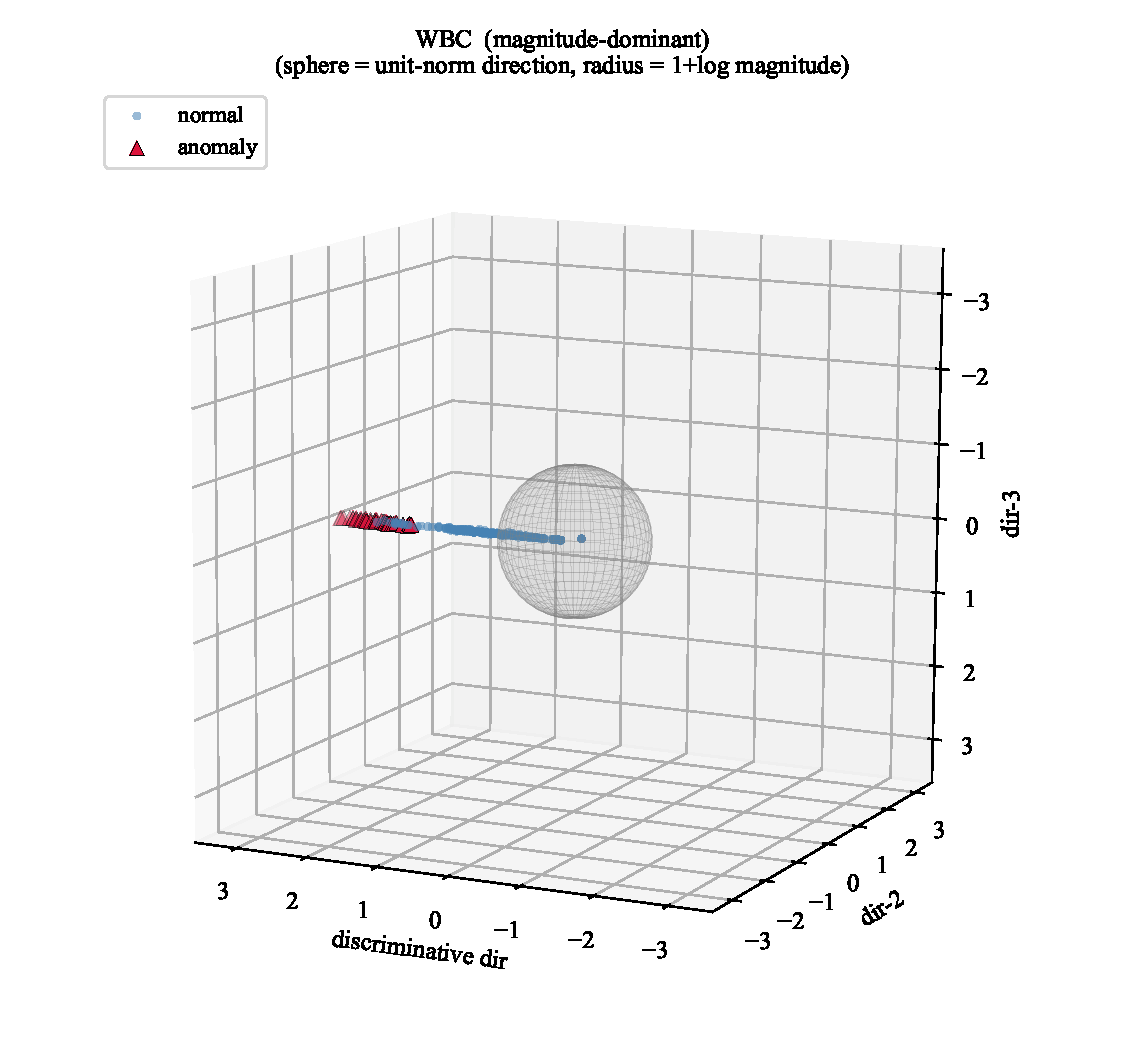
\includegraphics[width=\linewidth]{fig_sphere_wbc.pdf}\\[-2pt]
{\small (b) WBC --- magnitude-dominant}
\end{minipage}
\caption{Geometric view of the two complementary signals on the learned
representation. The grey sphere is the unit-norm (direction) manifold; a sample's
radius is $1+\log$ of its projection magnitude, so normal points ($\approx\!1$)
lie on the shell. \textbf{(a)} On Autos the anomalies remain on the shell but
concentrate in one angular region---separable by \emph{direction}, while their
magnitude is uninformative. \textbf{(b)} On WBC the anomalies are angularly
intermixed with the normal class yet bulge far outside the shell---separable only
by \emph{magnitude}. The angular (linear OC-SVM) detector handles~(a), the radial
(RBF OC-SVM) detector handles~(b), and the max-fusion is robust on both without
knowing the regime in advance. For visualization only, the principal in-sphere
axis is the normal/anomaly mean-difference direction (labels are used solely for
this projection, never for training or scoring).}
\label{fig:sphere}
\end{figure}

\subsection{Overall algorithm and complexity}
\label{subsec:algorithm}

Algorithm~\ref{alg:scmk} summarises the complete training and scoring pipeline.
The dominant per-mini-batch cost is the cross-kernel contrastive term,
$O\!\big(K^2 B^2 d\big)$ for the $\binom{K}{2}$ pairwise affinity matrices, while
the scatter regularizer contributes only $O(KBd)$. Embedding extraction over the
full data set is $O(NKdD)$. Scoring fits two OC-SVMs on the normal set: a linear
one on the $Kd$-dimensional embeddings and an RBF one on the $K$-dimensional
magnitude vectors; both scale with the number of support vectors, and the radial
detector is negligible since $K=5$. With a fixed small kernel bank, the method
retains the same asymptotic complexity as the contrastive backbone, so the
accuracy gains reported in the experiments come at no additional order-of-growth
cost.

\begin{algorithm}[t]
\caption{SCMK for one-class anomaly detection}
\label{alg:scmk}
\begin{algorithmic}[1]
\Require normal set $\Xnorm$, full set $\mathcal{X}$, kernel ratios
$\{r_k\}_{k=1}^{K}$, embedding dim.\ $d$, weight $\lambda$, batch size $B$,
epochs $T$, OC-SVM parameter $\nu$
\Ensure anomaly scores $\{a(\xx_i)\}_{i=1}^{N}$
\State $\mathrm{med}\gets$ median pairwise distance on $\Xnorm$
\Comment{Eq.~\eqref{eq:median}}
\State build kernels $\kappa_k$ with $t_k=r_k\,\mathrm{med}$
\Comment{Eq.~\eqref{eq:gaussian}}
\State initialise projection heads $\{\WW_k\}_{k=1}^{K}$
\For{$\mathrm{epoch}=1$ \textbf{to} $T$}
  \For{each mini-batch of $B$ samples from $\Xnorm$}
    \State $\hh_{k,i}\gets \WW_k\xx_i/\norm{\WW_k\xx_i}_2$ for all $k,i$
    \Comment{Eq.~\eqref{eq:embedding}}
    \State $\Lcross\gets$ cross-kernel InfoNCE over kernel pairs
    \Comment{Eqs.~\eqref{eq:affinity}--\eqref{eq:lcross}}
    \State $\Lscat\gets -\tfrac{1}{K}\sum_k\norm{\tfrac{1}{B}\sum_i\hh_{k,i}}_2^2$
    \Comment{Eq.~\eqref{eq:lscat}}
    \State update $\{\WW_k\}$ by a gradient step on
    $\Lcross+\lambda\Lscat$
    \Comment{Eq.~\eqref{eq:total}}
  \EndFor
\EndFor
\State $\zz_i\gets[\hh_{1,i};\dots;\hh_{K,i}]$,\ \
$\bm{r}_i\gets[\norm{\WW_1\xx_i};\dots;\norm{\WW_K\xx_i}]$ for all $\xx_i\in\mathcal{X}$
\Comment{Eqs.~\eqref{eq:concat},\eqref{eq:rmag}}
\State $s^{\mathrm{dir}}\gets$ linear OC-SVM on $\{\zz_i:y_i=0\}$;\ \
$s^{\mathrm{mag}}\gets$ RBF OC-SVM on $\{\bm{r}_i:y_i=0\}$
\Comment{Eq.~\eqref{eq:ocsvm}}
\State \Return $a(\xx_i)=\max\big(\widetilde{s}^{\mathrm{dir}}_i,\widetilde{s}^{\mathrm{mag}}_i\big)$
\Comment{Eq.~\eqref{eq:fuse}}
\end{algorithmic}
\end{algorithm}

%% ======================================================================
\section{Experiments}
\label{sec:exp}

\subsection{Experimental setup}
\label{subsec:exp-setup}

We evaluate on twenty public benchmark datasets\footnote{https://github.com/BELLoney/Outlier-detection} drawn from the UCI
repository, summarised in Table~\ref{tab:datasets}. They span a wide range of
sample sizes (101--5171), dimensionalities (6--154), anomaly rates
(1.9\%--25.2\%), scenarios, and cover numerical, nominal and mixed-type attributes, so that
robustness can be assessed across heterogeneous regimes. Following the
protocol adopted in recent anomaly-detection studies,
each dataset is split so that $50\%$ of the normal samples form the training set
while the remaining $50\%$ of normal samples together with all anomalies form the
test set. For the one-class methods---SCMK, Disent-AD, DeepSVDD, LMKAD, ICL and NeuTraLAD---we repeat it for three
random seeds ($0,1,2$), training on the training set and scoring on the test
set, and report the mean$_{\pm\text{std}}$ AUC; KFGOD and DFNO score samples transductively without a training
phase and run on the full set as in their native protocol.

We compare against seven recent outlier detectors: KFGOD~\cite{kfgod2024},
Disent-AD~\cite{disentad2025}, DeepSVDD~\cite{deepsvdd2018}, DFNO~\cite{dfno2024},
LMKAD~\cite{lmkad}, ICL~\cite{icl2022} and NeuTraLAD~\cite{neutralad2021}.
These include fuzzy-rough/neighbourhood (KFGOD, DFNO), deep one-class representation
(Disent-AD, DeepSVDD), multiple-kernel (LMKAD), self-supervised
contrastive and transformation (ICL, NeuTraLAD) paradigms, providing a strong and
diverse modern reference set.

The encoder of SCMK uses 5 Gaussian kernels with ratios $\{0.1,0.5,1,2,5\}$ and
bias-free linear heads, trained for $100$ epochs with Adam (learning rate
$0.01$, batch size $512$) on normal data only; the random seed is fixed to $42$.
The embedding dimension $d\!\in\!\{16,32,64,128,256\}$, the scatter weight
$\lambda\!\in\!\{0,0.1,1,10,100,1000\}$ and the OC-SVM parameter
$\nu\!\in\!\{0.01,0.05,0.1,0.2\}$ are selected per dataset. As is customary on
these benchmarks, every method---ours and all baselines---is reported at its best
hyper-parameter configuration, so the comparison reflects each detector's
attainable ceiling under a common protocol.

Detection quality is measured by the area under the ROC curve (AUC), with normal
samples labelled $0$ and anomalies $1$; higher is better.

\begin{table}[t]
\centering
\caption{The twenty benchmark datasets ($N$: samples, $D$: features,
$\rho$: anomaly rate).}
\label{tab:datasets}
\small
\setlength{\tabcolsep}{5pt}
\begin{tabular}{lrrr@{\hskip 18pt}lrrr}
\toprule
Dataset & $N$ & $D$ & $\rho$ & Dataset & $N$ & $D$ & $\rho$\\
\midrule
Vertebral    & 240  & 6   & 12.5\% & TicTacToe-69 & 695  & 27  & 9.9\%\\
Thyroid      & 3772 & 6   & 2.5\%  & WPBC         & 198  & 33  & 23.7\%\\
Ecoli        & 336  & 9   & 2.7\%  & Ionosphere   & 249  & 35  & 9.6\%\\
Glass        & 214  & 9   & 4.2\%  & Zoo          & 101  & 36  & 16.8\%\\
WBC          & 483  & 9   & 8.1\%  & Sick-72      & 3613 & 53  & 2.0\%\\
PageBlocks   & 5171 & 10  & 5.0\%  & Autos        & 205  & 54  & 12.2\%\\
Wine         & 129  & 13  & 7.8\%  & Annealing    & 798  & 56  & 5.3\%\\
Cardio       & 1831 & 21  & 9.6\%  & Lympho.      & 148  & 59  & 4.0\%\\
Cardiotoco.  & 1688 & 22  & 1.9\%  & Bands-6      & 318  & 62  & 1.9\%\\
TicTacToe-12 & 638  & 27  & 1.9\%  & Audiology    & 226  & 154 & 25.2\%\\
\bottomrule
\end{tabular}
\end{table}

\subsection{Comparison with recent detectors}
\label{subsec:exp-comparison}

Table~\ref{tab:comparison} reports the AUC of SCMK and the seven baselines. SCMK
attains the highest mean AUC, $0.914_{\pm0.022}$, exceeding the strongest single
competitor (DFNO, $0.863$) by $5.1$ points, the next one-class
methods LMKAD ($0.850$) and NeuTraLAD ($0.835$) by $6.4$ and $7.9$ points, and the
seven-method average ($0.824$) by $9.0$ points; it also has the lowest
across-seed standard deviation ($0.022$) among the one-class methods. SCMK holds
the best mean on $9$ of the $20$ datasets and wins $114$ of the $140$ pairwise
comparisons. The advantage is clearest where the baselines collectively struggle:
on Cardiotocography the best competitor reaches only $0.873$ against SCMK's $0.914$,
on Annealing $0.843$ against $0.877$, and on Audiology $0.970$ against
$0.982$. On the eleven datasets where SCMK does not hold the best mean it is usually
a close second---within $0.01$--$0.02$ of the leader (e.g.\ Thyroid $0.981$ vs.\
LMKAD/Disent-AD $0.985$, Cardio $0.969$ vs.\ LMKAD $0.973$, TicTacToe-12 $0.990$
vs.\ DFNO $1.000$, TicTacToe-69 $0.981$ vs.\ DFNO $0.999$); the only sizeable
shortfalls are Glass and Vertebral, where
Disent-AD's deep one-class encoder reaches $0.936$ and $0.785$. WBC is an angularly
indistinguishable case---used to motivate the magnitude branch in
Fig.~\ref{fig:sphere}---on which SCMK still attains $0.992$.
That SCMK leads on average across numerical, nominal and mixed-type data, with the
lowest across-seed standard deviation ($0.022$) among the one-class methods,
indicates that the kernel-fused, scatter-compacted representation generalises
robustly across feature types and random splits rather than exploiting a single
data regime. Per-dataset ROC curves for all
twenty datasets are given in Fig.~\ref{fig:roc_all}. The statistical
significance of this advantage is established in Section~\ref{subsec:exp-stat}.
As a threshold-based complement to the ranking-based AUC, Table~\ref{tab:gmean}
reports the maximum G-mean ($\sqrt{\mathrm{TPR}\cdot\mathrm{TNR}}$) of every
method; SCMK again attains the highest mean ($0.863$) and the most first-place
results, confirming that its advantage persists once a concrete decision
threshold is imposed and is not an artefact of the threshold-free AUC.

\begin{table*}[t]
\centering
\caption{AUC of SCMK against seven recent detectors on twenty datasets. The
one-class methods (SCMK, Disent-AD, DeepSVDD, LMKAD, ICL, NeuTraLAD) are reported 
as mean$_{\pm\text{std}}$ over three
random splits (seeds $0,1,2$). Best mean in each row is in \textbf{bold}.}
\label{tab:comparison}
\scriptsize
\setlength{\tabcolsep}{4pt}
\resizebox{\textwidth}{!}{
\begin{tabular}{lccccccc c}
\toprule
Dataset & KFGOD & Disent & DeepSVDD & DFNO & LMKAD & ICL & NeuTraLAD & SCMK\\
        & \cite{kfgod2024} & \cite{disentad2025} & \cite{deepsvdd2018}
        & \cite{dfno2024} & \cite{lmkad} & \cite{icl2022}
        & \cite{neutralad2021} & (ours)\\
\midrule
Vertebral    & $0.390$ & $\mathbf{0.785}_{\pm0.026}$ & $0.517_{\pm0.024}$ & $0.373$ & $0.655_{\pm0.067}$ & $0.345_{\pm0.060}$ & $0.627_{\pm0.043}$ & $0.735_{\pm0.092}$ \\
Thyroid      & $0.921$ & $\mathbf{0.985}_{\pm0.001}$ & $0.918_{\pm0.010}$ & $0.953$ & $\mathbf{0.985}_{\pm0.002}$ & $0.880_{\pm0.035}$ & $0.979_{\pm0.001}$ & $0.981_{\pm0.003}$ \\
WBC          & $\mathbf{0.997}$ & $0.964_{\pm0.004}$ & $0.864_{\pm0.024}$ & $\mathbf{0.997}$ & $0.992_{\pm0.003}$ & $0.967_{\pm0.008}$ & $0.808_{\pm0.034}$ & $0.992_{\pm0.007}$ \\
Glass        & $0.700$ & $\mathbf{0.936}_{\pm0.002}$ & $0.875_{\pm0.018}$ & $0.857$ & $0.588_{\pm0.069}$ & $0.855_{\pm0.038}$ & $0.875_{\pm0.012}$ & $0.853_{\pm0.058}$ \\
Ecoli        & $0.926$ & $0.834_{\pm0.041}$ & $0.761_{\pm0.042}$ & $0.905$ & $0.814_{\pm0.110}$ & $0.832_{\pm0.006}$ & $0.866_{\pm0.011}$ & $\mathbf{0.931}_{\pm0.010}$ \\
PageBlocks   & $0.957$ & $0.937_{\pm0.010}$ & $0.945_{\pm0.019}$ & $0.975$ & $0.995_{\pm0.001}$ & $0.989_{\pm0.004}$ & $\mathbf{0.996}_{\pm0.001}$ & $0.976_{\pm0.004}$ \\
Wine         & $0.887$ & $0.633_{\pm0.026}$ & $0.948_{\pm0.015}$ & $\mathbf{0.957}$ & $0.905_{\pm0.011}$ & $0.794_{\pm0.122}$ & $0.639_{\pm0.025}$ & $0.920_{\pm0.037}$ \\
Cardio       & $0.950$ & $0.744_{\pm0.018}$ & $0.935_{\pm0.016}$ & $0.914$ & $\mathbf{0.973}_{\pm0.003}$ & $0.896_{\pm0.029}$ & $0.960_{\pm0.003}$ & $0.969_{\pm0.002}$ \\
Cardiotoco.  & $0.870$ & $0.804_{\pm0.013}$ & $0.839_{\pm0.013}$ & $0.809$ & $0.873_{\pm0.014}$ & $0.751_{\pm0.102}$ & $0.754_{\pm0.024}$ & $\mathbf{0.914}_{\pm0.008}$ \\
TicTacToe-12 & $0.898$ & $0.811_{\pm0.111}$ & $0.750_{\pm0.043}$ & $\mathbf{1.000}$ & $0.938_{\pm0.004}$ & $0.694_{\pm0.067}$ & $0.823_{\pm0.009}$ & $0.990_{\pm0.003}$ \\
TicTacToe-69 & $0.690$ & $0.766_{\pm0.020}$ & $0.626_{\pm0.028}$ & $\mathbf{0.999}$ & $0.707_{\pm0.037}$ & $0.739_{\pm0.042}$ & $0.815_{\pm0.010}$ & $0.981_{\pm0.018}$ \\
WPBC         & $0.494$ & $0.631_{\pm0.008}$ & $0.532_{\pm0.004}$ & $0.556$ & $0.470_{\pm0.016}$ & $0.564_{\pm0.039}$ & $0.478_{\pm0.070}$ & $\mathbf{0.653}_{\pm0.090}$ \\
Ionosphere   & $0.999$ & $0.954_{\pm0.017}$ & $\mathbf{1.000}_{\pm0.001}$ & $\mathbf{1.000}$ & $\mathbf{1.000}_{\pm0.000}$ & $\mathbf{1.000}_{\pm0.000}$ & $\mathbf{1.000}_{\pm0.000}$ & $\mathbf{1.000}_{\pm0.000}$ \\
Zoo          & $0.457$ & $0.883_{\pm0.009}$ & $0.939_{\pm0.064}$ & $0.934$ & $0.842_{\pm0.047}$ & $0.959_{\pm0.040}$ & $0.968_{\pm0.050}$ & $\mathbf{0.969}_{\pm0.020}$ \\
Sick-72      & $0.760$ & $0.815_{\pm0.009}$ & $0.774_{\pm0.038}$ & $0.833$ & $\mathbf{0.846}_{\pm0.049}$ & $0.582_{\pm0.174}$ & $0.818_{\pm0.003}$ & $0.828_{\pm0.016}$ \\
Autos        & $0.625$ & $0.722_{\pm0.035}$ & $0.679_{\pm0.048}$ & $0.623$ & $0.804_{\pm0.021}$ & $0.725_{\pm0.083}$ & $0.707_{\pm0.049}$ & $\mathbf{0.822}_{\pm0.019}$ \\
Annealing    & $0.783$ & $0.735_{\pm0.009}$ & $0.795_{\pm0.044}$ & $0.759$ & $0.842_{\pm0.018}$ & $0.758_{\pm0.062}$ & $0.843_{\pm0.016}$ & $\mathbf{0.877}_{\pm0.008}$ \\
Lympho.      & $0.988$ & $0.745_{\pm0.017}$ & $0.931_{\pm0.037}$ & $0.998$ & $0.995_{\pm0.006}$ & $0.947_{\pm0.021}$ & $0.976_{\pm0.007}$ & $\mathbf{0.999}_{\pm0.001}$ \\
Bands-6      & $0.822$ & $0.677_{\pm0.012}$ & $0.936_{\pm0.047}$ & $0.909$ & $0.941_{\pm0.025}$ & $0.789_{\pm0.033}$ & $\mathbf{0.953}_{\pm0.021}$ & $0.914_{\pm0.044}$ \\
Audiology    & $0.831$ & $0.887_{\pm0.020}$ & $0.970_{\pm0.009}$ & $0.903$ & $0.831_{\pm0.079}$ & $0.681_{\pm0.039}$ & $0.819_{\pm0.074}$ & $\mathbf{0.982}_{\pm0.008}$ \\
\midrule
\textbf{Average} & $0.797$ & $0.812_{\pm0.020}$ & $0.827_{\pm0.027}$ & $0.863$ & $0.850_{\pm0.029}$ & $0.787_{\pm0.050}$ & $0.835_{\pm0.023}$ & $\mathbf{0.914}_{\pm0.022}$ \\
\bottomrule
\end{tabular}
}
\end{table*}

\begin{table*}[t]
\centering
\caption{Maximum G-mean ($\sqrt{\mathrm{TPR}\cdot\mathrm{TNR}}$) of SCMK against seven recent
detectors on twenty datasets, as a threshold-based complement to the AUC in
Table~\ref{tab:comparison}. The one-class methods (SCMK, Disent-AD, DeepSVDD, LMKAD, ICL,
NeuTraLAD) are reported as mean$_{\pm\text{std}}$ over three random splits (seeds $0,1,2$);
KFGOD and DFNO are transductive on the full set (single-valued). Best mean in each row is in
\textbf{bold}.}
\label{tab:gmean}
\scriptsize
\setlength{\tabcolsep}{4pt}
\resizebox{\textwidth}{!}{
\begin{tabular}{lccccccc c}
\toprule
Dataset & KFGOD & Disent & DeepSVDD & DFNO & LMKAD & ICL & NeuTraLAD & SCMK\\
\midrule
Vertebral    & $0.454$ & $\mathbf{0.741}_{\pm0.022}$ & $0.533_{\pm0.005}$ & $0.436$ & $0.661_{\pm0.047}$ & $0.423_{\pm0.055}$ & $0.624_{\pm0.052}$ & $0.669_{\pm0.106}$ \\
Thyroid      & $0.864$ & $\mathbf{0.952}_{\pm0.003}$ & $0.855_{\pm0.030}$ & $0.909$ & $0.947_{\pm0.005}$ & $0.882_{\pm0.051}$ & $0.935_{\pm0.002}$ & $0.936_{\pm0.007}$ \\
WBC          & $\mathbf{0.992}$ & $0.926_{\pm0.015}$ & $0.797_{\pm0.025}$ & $0.985$ & $0.986_{\pm0.004}$ & $0.937_{\pm0.004}$ & $0.816_{\pm0.030}$ & $0.985_{\pm0.003}$ \\
Glass        & $0.752$ & $0.892_{\pm0.025}$ & $0.896_{\pm0.011}$ & $\mathbf{0.897}$ & $0.613_{\pm0.024}$ & $0.843_{\pm0.044}$ & $0.889_{\pm0.003}$ & $0.861_{\pm0.073}$ \\
Ecoli        & $0.878$ & $0.798_{\pm0.054}$ & $0.781_{\pm0.059}$ & $0.879$ & $0.821_{\pm0.101}$ & $0.866_{\pm0.008}$ & $0.866_{\pm0.018}$ & $\mathbf{0.890}_{\pm0.024}$ \\
PageBlocks   & $0.895$ & $0.872_{\pm0.009}$ & $0.874_{\pm0.031}$ & $0.948$ & $\mathbf{0.987}_{\pm0.002}$ & $0.974_{\pm0.005}$ & $0.979_{\pm0.001}$ & $0.953_{\pm0.003}$ \\
Wine         & $0.879$ & $0.641_{\pm0.046}$ & $0.935_{\pm0.012}$ & $\mathbf{0.948}$ & $0.857_{\pm0.035}$ & $0.797_{\pm0.107}$ & $0.673_{\pm0.018}$ & $0.720_{\pm0.227}$ \\
Cardio       & $0.890$ & $0.681_{\pm0.009}$ & $0.865_{\pm0.017}$ & $0.879$ & $\mathbf{0.924}_{\pm0.004}$ & $0.852_{\pm0.052}$ & $0.903_{\pm0.008}$ & $0.910_{\pm0.010}$ \\
Cardiotoco.  & $0.835$ & $0.781_{\pm0.036}$ & $0.793_{\pm0.006}$ & $0.778$ & $0.820_{\pm0.009}$ & $0.716_{\pm0.082}$ & $0.719_{\pm0.030}$ & $\mathbf{0.836}_{\pm0.022}$ \\
TicTacToe-12 & $0.821$ & $0.795_{\pm0.093}$ & $0.714_{\pm0.030}$ & $\mathbf{1.000}$ & $0.933_{\pm0.004}$ & $0.710_{\pm0.072}$ & $0.811_{\pm0.013}$ & $0.747_{\pm0.267}$ \\
TicTacToe-69 & $0.677$ & $0.751_{\pm0.011}$ & $0.605_{\pm0.020}$ & $\mathbf{0.990}$ & $0.714_{\pm0.027}$ & $0.689_{\pm0.028}$ & $0.774_{\pm0.015}$ & $0.965_{\pm0.034}$ \\
WPBC         & $0.539$ & $0.629_{\pm0.022}$ & $0.554_{\pm0.012}$ & $0.561$ & $0.505_{\pm0.009}$ & $0.594_{\pm0.051}$ & $0.517_{\pm0.067}$ & $\mathbf{0.634}_{\pm0.076}$ \\
Ionosphere   & $0.993$ & $0.903_{\pm0.031}$ & $0.997_{\pm0.005}$ & $\mathbf{1.000}$ & $\mathbf{1.000}_{\pm0.000}$ & $0.997_{\pm0.005}$ & $\mathbf{1.000}_{\pm0.000}$ & $0.996_{\pm0.008}$ \\
Zoo          & $0.529$ & $0.843_{\pm0.051}$ & $0.935_{\pm0.047}$ & $0.911$ & $0.802_{\pm0.038}$ & $0.922_{\pm0.039}$ & $\mathbf{0.963}_{\pm0.033}$ & $0.913_{\pm0.048}$ \\
Sick-72      & $0.744$ & $0.811_{\pm0.005}$ & $0.726_{\pm0.043}$ & $\mathbf{0.821}$ & $0.782_{\pm0.049}$ & $0.584_{\pm0.171}$ & $0.799_{\pm0.015}$ & $0.816_{\pm0.010}$ \\
Autos        & $0.624$ & $0.716_{\pm0.014}$ & $0.684_{\pm0.046}$ & $0.613$ & $\mathbf{0.806}_{\pm0.021}$ & $0.720_{\pm0.073}$ & $0.692_{\pm0.059}$ & $0.780_{\pm0.021}$ \\
Annealing    & $0.768$ & $0.697_{\pm0.012}$ & $0.751_{\pm0.025}$ & $0.743$ & $0.800_{\pm0.035}$ & $0.707_{\pm0.049}$ & $0.792_{\pm0.013}$ & $\mathbf{0.812}_{\pm0.025}$ \\
Lympho.      & $0.979$ & $0.717_{\pm0.018}$ & $0.919_{\pm0.033}$ & $0.993$ & $0.988_{\pm0.015}$ & $0.915_{\pm0.011}$ & $0.944_{\pm0.004}$ & $\mathbf{0.995}_{\pm0.004}$ \\
Bands-6      & $0.775$ & $0.692_{\pm0.030}$ & $0.927_{\pm0.073}$ & $0.864$ & $\mathbf{0.940}_{\pm0.029}$ & $0.763_{\pm0.043}$ & $0.932_{\pm0.038}$ & $0.896_{\pm0.045}$ \\
Audiology    & $0.754$ & $0.825_{\pm0.017}$ & $0.933_{\pm0.021}$ & $0.837$ & $0.784_{\pm0.080}$ & $0.653_{\pm0.016}$ & $0.806_{\pm0.066}$ & $\mathbf{0.948}_{\pm0.022}$ \\
\midrule
\textbf{Average} & $0.782$ & $0.783_{\pm0.026}$ & $0.804_{\pm0.028}$ & $0.850$ & $0.834_{\pm0.027}$ & $0.777_{\pm0.048}$ & $0.822_{\pm0.024}$ & $\mathbf{0.863}_{\pm0.052}$ \\
\bottomrule
\end{tabular}
}
\end{table*}

\begin{figure*}[p]
\centering
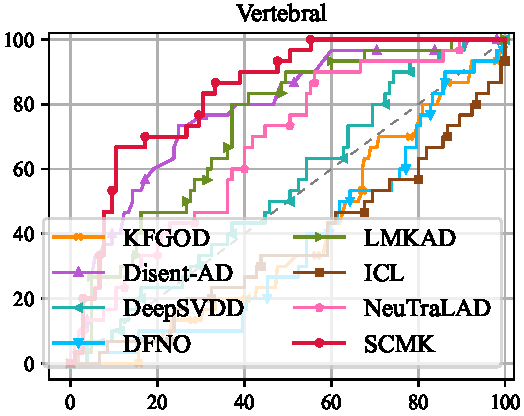
\includegraphics[width=0.24\textwidth]{roc_figs/new/vertebral_ROC.pdf}\hfill
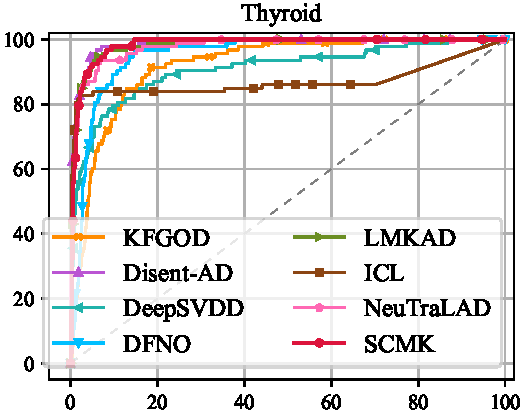
\includegraphics[width=0.24\textwidth]{roc_figs/new/thyroid_ROC.pdf}\hfill

\includegraphics[width=0.24\textwidth]{roc_figs/new/ecoli_ROC.pdf}\hfill

\includegraphics[width=0.24\textwidth]{roc_figs/new/glass_ROC.pdf}\\[4pt]
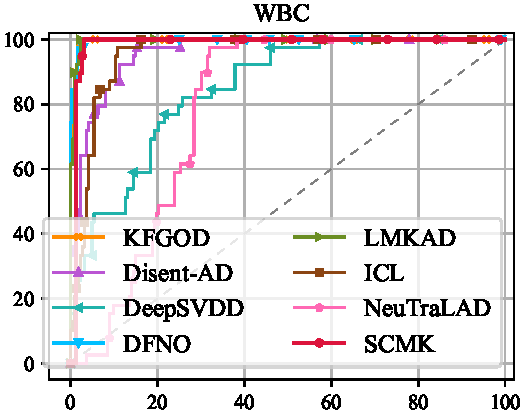
\includegraphics[width=0.24\textwidth]{roc_figs/new/wbc_malignant_39_variant1_ROC.pdf}\hfill
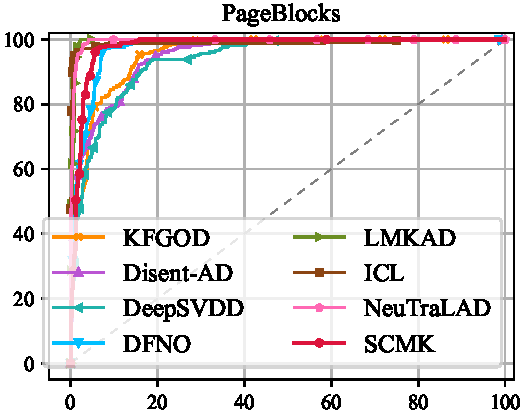
\includegraphics[width=0.24\textwidth]{roc_figs/new/pageblocks_1_258_variant1_ROC.pdf}\hfill
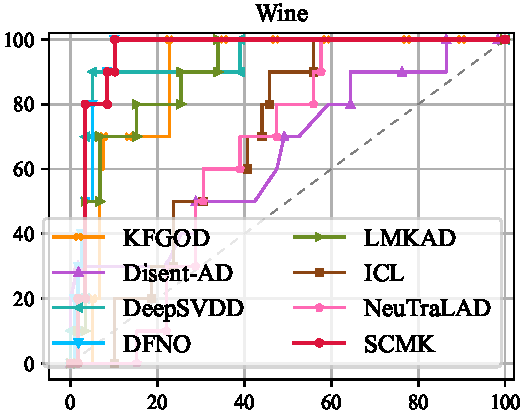
\includegraphics[width=0.24\textwidth]{roc_figs/new/wine_ROC.pdf}\hfill

\includegraphics[width=0.24\textwidth]{roc_figs/new/cardio_ROC.pdf}\\[4pt]

\includegraphics[width=0.24\textwidth]{roc_figs/new/cardiotocography_2and3_33_variant1_ROC.pdf}\hfill
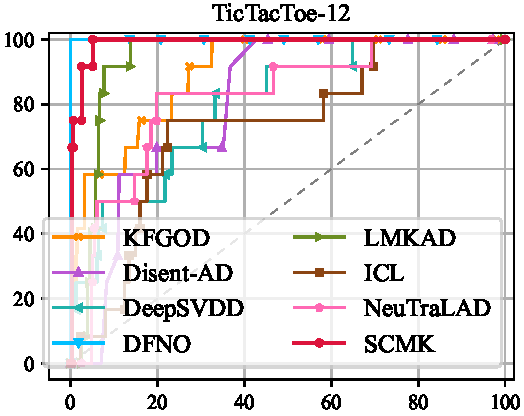
\includegraphics[width=0.24\textwidth]{roc_figs/new/tic_tac_toe_negative_12_variant1_ROC.pdf}\hfill
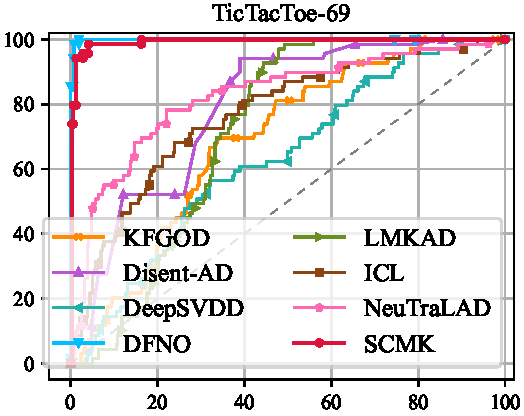
\includegraphics[width=0.24\textwidth]{roc_figs/new/tic_tac_toe_negative_69_variant1_ROC.pdf}\hfill
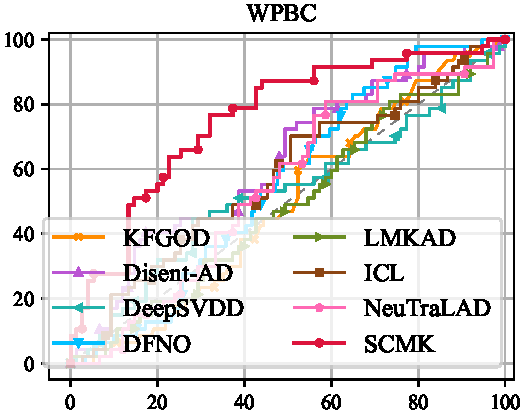
\includegraphics[width=0.24\textwidth]{roc_figs/new/wpbc_variant1_ROC.pdf}\\[4pt]

\includegraphics[width=0.24\textwidth]{roc_figs/new/ionosphere_b_24_variant1_ROC.pdf}\hfill
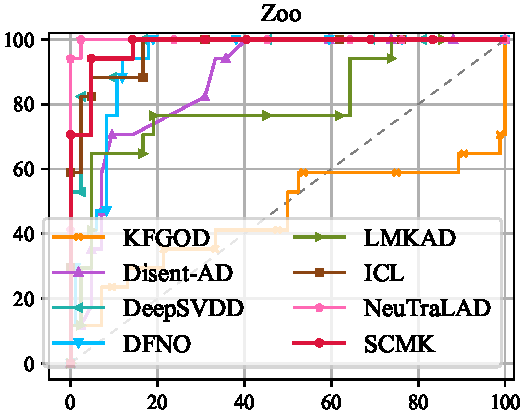
\includegraphics[width=0.24\textwidth]{roc_figs/new/zoo_variant1_ROC.pdf}\hfill
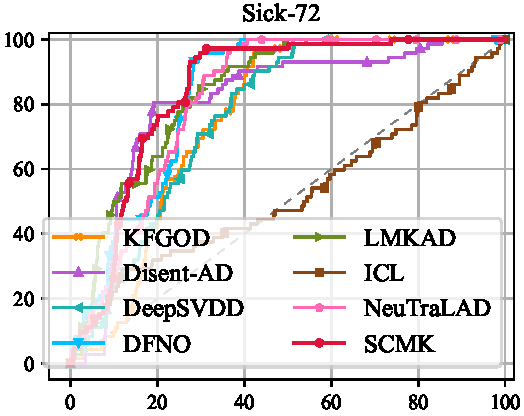
\includegraphics[width=0.24\textwidth]{roc_figs/new/sick_sick_72_variant1_ROC.pdf}\hfill

\includegraphics[width=0.24\textwidth]{roc_figs/new/autos_variant1_ROC.pdf}\\[4pt]

\includegraphics[width=0.24\textwidth]{roc_figs/new/annealing_variant1_ROC.pdf}\hfill

\includegraphics[width=0.24\textwidth]{roc_figs/new/lymphography_ROC.pdf}\hfill

\includegraphics[width=0.24\textwidth]{roc_figs/new/bands_band_6_variant1_ROC.pdf}\hfill

\includegraphics[width=0.24\textwidth]{roc_figs/new/audiology_variant1_ROC.pdf}
\caption{Per-dataset ROC curves on the twenty datasets.}
\label{fig:roc_all}
\end{figure*}

\subsection{Runtime evaluation}
\label{subsec:exp-runtime}

Because SCMK forms $\binom{K}{2}$ pairwise cross-kernel affinity matrices per
mini-batch and maintains $K$ projection heads, its cost warrants an empirical
check rather than an asymptotic argument alone. We therefore measure the actual
wall-clock \emph{training} and \emph{inference} time of SCMK against the baselines
under a unified protocol: the same GPU, the seed-2 split, a single per-dataset
configuration, one CUDA warm-up, and the median of repeated inference passes.
Training is the fit on the normal training set; inference is scoring the test set.
The transductive detectors (KFGOD, DFNO) have no separate training phase, and to
isolate the multiple-kernel overhead we also time the single-kernel variant
SCMK$_{K=1}$. KFGOD and LMKAD are timed through their official code; the results
are summarised in Fig.~\ref{fig:runtime} (means over the twenty datasets).

\paragraph{The multiple-kernel overhead is real but bounded.} SCMK trains in
$3.07$\,s on average versus $0.23$\,s for SCMK$_{K=1}$, so the $\binom{K}{2}$
affinity computation with $K=5$ multiplies training time by roughly $13\times$.
In absolute terms, however, SCMK remains firmly mid-pack among the deep detectors:
it is faster than NeuTraLAD ($4.80$\,s) and about $5\times$ faster than ICL
($15.25$\,s), and comparable to Disent-AD ($2.66$\,s), while the lighter DeepSVDD
($1.04$\,s) and the kernel one-class LMKAD ($0.35$\,s) are cheaper. SCMK is thus
not an outlier in training cost, and the overhead buys the multi-scale
representation that drives its accuracy.

\paragraph{Inference is near-instant and scales gracefully.} At test time SCMK
scores a dataset in $11$\,ms on average---among the fastest methods, since
inference is a single forward pass plus two linear/RBF OC-SVM evaluations. The two
transductive baselines are orders of magnitude slower and, being $O(n^2)$, degrade
sharply with size: on the largest test set (PageBlocks, $n\!=\!2715$) SCMK infers
in $0.13$\,s whereas DFNO takes $2.47$\,s and KFGOD $27.97$\,s. SCMK therefore
pays a modest one-off training premium for its kernel bank yet is highly efficient
to deploy, in contrast to transductive methods that must recompute over the whole
data at every query.

\begin{figure*}[t]
\centering
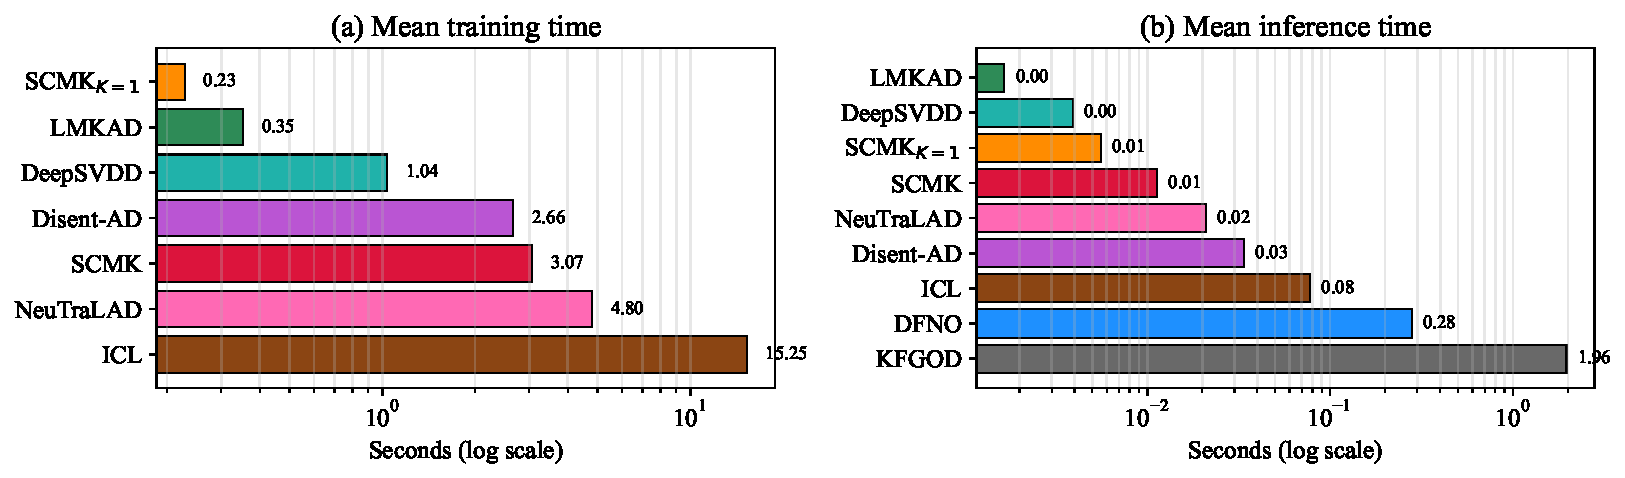
\includegraphics[width=\textwidth]{fig_runtime.pdf}
\caption{Mean \textbf{(a)} training and \textbf{(b)} inference time (seconds,
log scale) over the twenty datasets on a single GPU. SCMK$_{K=1}$ is the
single-kernel variant; KFGOD and DFNO are transductive and appear only under
inference. SCMK's multiple-kernel training cost ($3.07$\,s) stays below NeuTraLAD
and ICL, and its inference ($11$\,ms) is among the fastest---far below the
transductive KFGOD ($1.96$\,s) and DFNO ($0.28$\,s).}
\label{fig:runtime}
\end{figure*}

\subsection{Statistical significance}
\label{subsec:exp-stat}

To confirm that the advantage in Table~\ref{tab:comparison} is statistically
significant rather than incidental, we follow the standard protocol of
Dem\v{s}ar~\cite{demsar2006}: a Friedman test across all eight methods (using each
method's per-dataset mean AUC), followed by the Nemenyi post-hoc test rendered as
a critical-difference (CD) diagram.

The Friedman test strongly rejects the null hypothesis that the eight methods
perform equally ($\chi^2_F=34.98$, $p=1.1\times10^{-5}$; Iman--Davenport
$F=6.33$). Fig.~\ref{fig:cd} shows the CD diagram at significance level
$\alpha=0.05$ ($\mathrm{CD}=2.35$). SCMK attains the best mean rank, $2.23$, and is
separated by more than the critical difference from four of the seven baselines
(DeepSVDD $5.25$, KFGOD $5.35$, DisentAD $5.40$, ICL $5.95$). The three strongest
competitors---LMKAD ($3.78$), DFNO ($3.83$) and NeuTraLAD ($4.23$)---fall within
the critical difference of SCMK, so the conservative Nemenyi test places them in
the same top cluster; the pairwise analysis below resolves this finer ordering and
still finds SCMK significantly ahead of all three.

\begin{figure}[t]
\centering
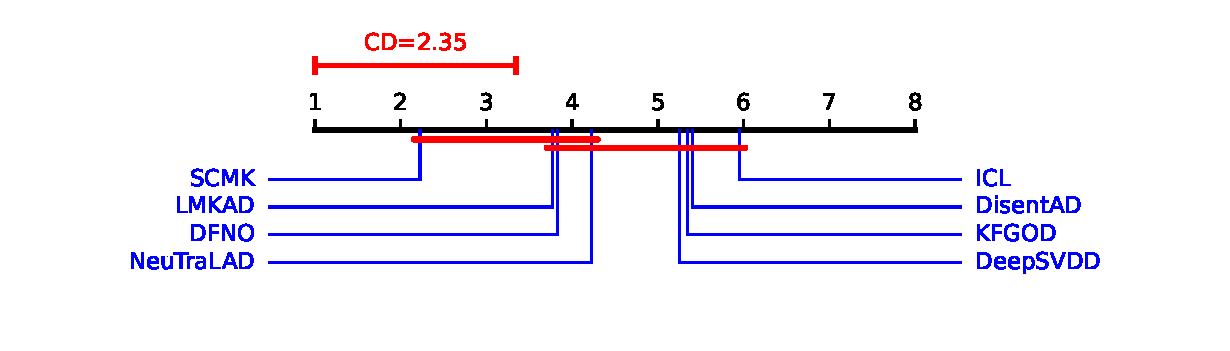
\includegraphics[width=0.92\linewidth]{cd_diagram.pdf}
\caption{Critical-difference diagram (Nemenyi post-hoc, $\alpha=0.05$,
$\mathrm{CD}=2.35$) over the twenty datasets, using each method's per-dataset mean
AUC. Lower rank (towards the right) is better; methods not connected by a thick bar
are not significantly different. SCMK (mean rank $2.23$) has the best rank;
DisentAD, DeepSVDD, KFGOD and ICL are significantly worse, while LMKAD, DFNO and
NeuTraLAD share its top cluster.}
\label{fig:cd}
\end{figure}

We further corroborate this with pairwise one-sided Wilcoxon signed-rank tests
of SCMK against each baseline, applying the Holm correction for multiple
comparisons (Table~\ref{tab:wilcoxon}). SCMK wins against every baseline on a
majority of datasets ($13$--$19$ of $20$), and all Holm-adjusted $p$-values are
below $0.05$ (and below $0.01$ for six of the seven), so the improvement is
significant in all seven comparisons. The
margin is largest over the weaker baselines ($p<10^{-3}$ for KFGOD, DisentAD,
DeepSVDD and ICL) and, while smaller, remains significant against the three
top-cluster methods that the Nemenyi test could not separate---LMKAD ($14/20$,
Holm $p=8.9\times10^{-3}$), DFNO ($13/20$, $1.7\times10^{-2}$) and NeuTraLAD
($16/20$, $3.8\times10^{-3}$).

\begin{table}[t]
\centering
\caption{Pairwise comparison of SCMK against each baseline (ordered by average
rank): mean rank, number of datasets on which SCMK wins, and one-sided Wilcoxon
signed-rank $p$-values before and after Holm correction.
$^{***}$:\ $p<0.001$; $^{**}$:\ $p<0.01$; $^{*}$:\ $p<0.05$.}
\label{tab:wilcoxon}
\small
\setlength{\tabcolsep}{6pt}
\begin{tabular}{lcccc}
\toprule
Method & Avg.\ rank & SCMK wins & Wilcoxon $p$ & Holm $p$\\
\midrule
LMKAD~\cite{lmkad}        & 3.78 & 14/20 & $4.5\times10^{-3}$ & $8.9\times10^{-3\;**}$\\
DFNO~\cite{dfno2024}      & 3.83 & 13/20 & $1.7\times10^{-2}$ & $1.7\times10^{-2\;*}$\\
NeuTraLAD~\cite{neutralad2021} & 4.23 & 16/20 & $1.3\times10^{-3}$ & $3.8\times10^{-3\;**}$\\
DeepSVDD~\cite{deepsvdd2018} & 5.25 & 17/20 & $6.7\times10^{-5}$ & $3.3\times10^{-4\;***}$\\
KFGOD~\cite{kfgod2024}    & 5.35 & 19/20 & $2.9\times10^{-6}$ & $2.0\times10^{-5\;***}$\\
DisentAD~\cite{disentad2025} & 5.40 & 17/20 & $1.6\times10^{-4}$ & $6.4\times10^{-4\;***}$\\
ICL~\cite{icl2022}        & 5.95 & 18/20 & $1.3\times10^{-5}$ & $8.0\times10^{-5\;***}$\\
\midrule
\textbf{SCMK (ours)} & \textbf{2.23} & --- & --- & ---\\
\bottomrule
\end{tabular}
\end{table}

\subsection{Parameter sensitivity}
\label{subsec:exp-sensitivity}

We finally probe how SCMK responds to its three hyper-parameters---the embedding
dimension $d$, the scatter weight $\lambda$, and the OC-SVM parameter $\nu$---by
varying one at a time on the twenty datasets and averaging the test AUC over the
three seeds $\{0,1,2\}$. When a parameter is varied, the remaining ones are set to
their per-dataset optimum, so each curve reports the AUC attainable at that
setting (shaded band: standard deviation across datasets). Fig.~\ref{fig:sens}
summarises the result.

\paragraph{$\lambda$ is the only sensitive knob.} The scatter weight has by far
the widest span (mean AUC ranging over $0.165$) and a distinctly non-monotone
profile: disabling the penalty ($\lambda=0$) gives $0.797$, a \emph{small} weight
is actively harmful ($0.724$ at $\lambda=0.1$, $0.742$ at $\lambda=1$), and only
once $\lambda\!\ge\!10$ does the term pay off, peaking at $0.890$ ($\lambda=100$)
and staying flat to $\lambda=1000$. A weak scatter penalty perturbs the
cross-kernel consistency objective without supplying enough intra-class
compactness to compensate; a sufficiently strong one delivers the compactness that
one-class detection needs. This corroborates the ablation of
Section~\ref{subsec:exp-ablation} and pins the useful range to $\lambda\in[10,1000]$.

\paragraph{$d$ and $\nu$ are robust.} By contrast, the embedding dimension is
nearly flat (span $0.032$): any $d\in\{32,\dots,256\}$ performs within $0.01$ of
the $d=128$ optimum, so SCMK needs no careful width tuning. The OC-SVM $\nu$ is
likewise stable (span $0.038$): AUC is essentially constant for $\nu\le0.2$ and
declines only gently beyond, favouring a small $\nu$. Overall, SCMK works
out-of-the-box for $d$ and $\nu$; the single design choice that matters is giving
the scatter term a large enough weight.

\begin{figure*}[t]
\centering
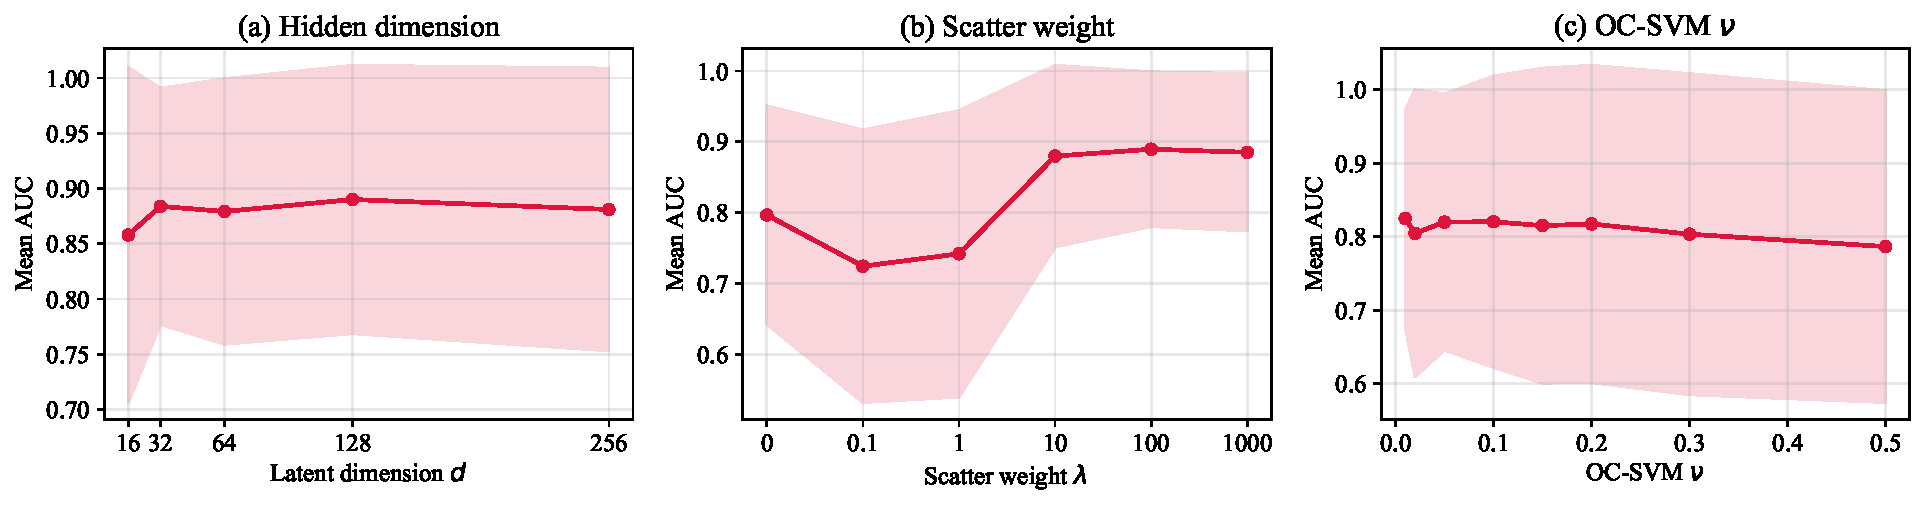
\includegraphics[width=\textwidth]{fig_sensitivity.pdf}
\caption{Parameter sensitivity of SCMK on the twenty datasets (mean test AUC over
seeds $\{0,1,2\}$; shaded band: standard deviation across datasets). \textbf{(a)}
Embedding dimension $d$ and \textbf{(c)} OC-SVM $\nu$ are flat (span $0.03$--$0.04$),
so SCMK is insensitive to them. \textbf{(b)} The scatter weight $\lambda$ is the
only sensitive parameter: a weak penalty ($\lambda\!\le\!1$) underperforms even
$\lambda=0$, while $\lambda\!\ge\!10$ is needed for the intra-class compactness
that drives detection, plateauing over $[10,1000]$.}
\label{fig:sens}
\end{figure*}

\subsection{Ablation study}
\label{subsec:exp-ablation}

To isolate the contribution of each component we ablate four design choices on
eight representative datasets that deliberately span both detection regimes
(angularly separable, e.g.\ Cardio and Ionosphere; magnitude-separable, e.g.\
WBC and Autos). The variants are: removing the scatter loss
(\emph{w/o $\Lscat$}, i.e.\ $\lambda=0$); removing the cross-kernel contrastive
loss (\emph{w/o $\Lcross$}); replacing the five-kernel bank with a single kernel
(\emph{single-kernel}); and restricting the detector to one signal
(\emph{dir.\ only}, the angular score; \emph{mag.\ only}, the radial score).
Table~\ref{tab:ablation} reports the results, and the average row quantifies the
mean impact of each removal.

\begin{table}[t]
\centering
\caption{Ablation of the four core components (AUC). Best result in each row is
in \textbf{bold}. The average row shows that the full model is the most robust
overall, even though a single-signal variant occasionally peaks on a dataset of
its favoured regime.}
\label{tab:ablation}
\small
\setlength{\tabcolsep}{4.5pt}
\begin{tabular}{lcccccc}
\toprule
Dataset & Full & w/o $\Lscat$ & w/o $\Lcross$ & single-kernel
        & dir.\ only & mag.\ only\\
\midrule
Ecoli      & 0.933 & 0.874 & 0.931 & 0.858 & 0.902 & \textbf{0.969}\\
WBC        & 0.985 & 0.981 & 0.984 & 0.986 & 0.586 & \textbf{0.998}\\
Vowels     & \textbf{0.978} & 0.330 & 0.977 & 0.963 & 0.909 & 0.906\\
Cardio     & 0.967 & 0.901 & 0.844 & 0.703 & \textbf{0.967} & 0.918\\
Autos      & 0.805 & 0.696 & 0.802 & \textbf{0.837} & 0.830 & 0.763\\
Ionosphere & \textbf{1.000} & 0.866 & \textbf{1.000} & \textbf{1.000} & \textbf{1.000} & 0.976\\
Bands-6    & 0.957 & 0.517 & 0.954 & 0.920 & \textbf{0.967} & 0.917\\
Sonar      & \textbf{0.984} & 0.794 & 0.978 & \textbf{0.984} & 0.978 & 0.951\\
\midrule
\textbf{Average} & \textbf{0.951} & 0.745 & 0.934 & 0.906 & 0.892 & 0.925\\
\bottomrule
\end{tabular}
\end{table}

\paragraph{Scatter loss is the dominant component.}
Removing the scatter regularizer ($\lambda=0$) causes by far the largest
degradation, $-0.206$ on average, collapsing Vowels from $0.978$ to $0.330$ and
Bands-6 from $0.957$ to $0.517$. This confirms the central thesis of the paper:
cross-kernel \emph{consistency} alone does not deliver the intra-class
\emph{compactness} that one-class detection requires, and the scatter penalty is
what supplies it.

\paragraph{Dual-signal fusion is what makes the detector robust.}
The two single-signal variants each excel on one regime but \emph{collapse} on
the other. The angular detector (\emph{dir.\ only}) matches the full model on
angularly separable data (Cardio $0.967$, Ionosphere $1.000$, Sonar $0.978$) yet
falls to $0.586$ on WBC, where normal and malignant cells are nearly
indistinguishable in angle; conversely the radial detector (\emph{mag.\ only})
handles WBC ($0.998$) but drops to $0.763$ on Autos. The fused detector never
collapses and attains the highest mean ($0.951$) \emph{without} any prior
knowledge of which signal is informative. The occasional cases where a single
signal slightly exceeds the full model on its own favoured dataset (e.g.\
\emph{dir.\ only} on Cardio) are precisely offset by its collapse elsewhere ---
direct evidence that the fusion, not either signal alone, is the robust choice.

\paragraph{Multi-kernel and contrastive terms.}
Reducing the bank to a single kernel costs $-0.045$ on average but is strongly
dataset-dependent: it removes $0.26$ AUC on Cardio, where multi-scale structure
is essential, while leaving datasets with a single dominant scale almost
unaffected. Removing the cross-kernel contrastive loss costs the least on
average ($-0.017$); once the scatter penalty is present, the additional
consistency constraint contributes only modestly to accuracy, yet it remains
important as the uniformity counterweight that prevents representational collapse
(Section~\ref{subsec:joint}).

%% ======================================================================
\section{Conclusion and future work}
\label{sec:conclusion}

This paper presented SCMK, a scatter-regularized cross-multi-kernel contrastive
framework for one-class anomaly detection. SCMK reconciles a bank of multi-scale
Gaussian kernels through a cross-kernel InfoNCE objective that treats the kernel
index as the contrastive view, and it compacts the normal class in every
kernel-induced space through a multi-kernel scatter regularizer that we proved to
be equivalent, up to an additive constant, to the average within-class scatter and
to the one-class instance of centroid multiple-kernel $k$-means. The learned
representation is exploited by a lightweight dual-signal detector that fuses an
angular (linear OC-SVM) and a radial (RBF OC-SVM) score, recovering the
discriminative information that $\ell_2$ normalization alone discards. Across
twenty benchmark datasets and seven recent detectors, SCMK attained the highest
mean AUC ($0.914$) and the best mean rank ($2.23$), with the improvement confirmed
significant by Friedman--Nemenyi and Holm-corrected Wilcoxon tests; ablation and
sensitivity studies isolated the scatter term as the dominant component and the
dual-signal fusion as the source of robustness, while the runtime analysis showed
that the multiple-kernel training premium is bounded and inference stays
near-instant.

Several directions remain open. The kernel bank currently uses a fixed
median-calibrated Gaussian family; learning the bandwidths, or extending to richer
kernel families, could adapt the multi-resolution prior to each dataset. The
present protocol assumes an uncontaminated normal training set, so relaxing SCMK to
tolerate label noise or a small anomaly contamination during training is a natural
next step. Finally, because inference reduces to a forward pass and two OC-SVM
evaluations rather than a transductive recomputation, extending SCMK to streaming
and high-dimensional (e.g.\ image or graph) settings is a promising avenue for
scaling the method beyond tabular anomaly detection.

%% ======================================================================
%% Bibliography
\begin{thebibliography}{00}

%% --- One-class and deep anomaly detection ---
\bibitem{scholkopf2001ocsvm}
B.~Sch\"olkopf, J.~C.~Platt, J.~Shawe-Taylor, A.~J.~Smola, R.~C.~Williamson,
\textit{Estimating the support of a high-dimensional distribution},
Neural Computation 13~(7) (2001) 1443--1471.

\bibitem{tax2004svdd}
D.~M.~J.~Tax, R.~P.~W.~Duin,
\textit{Support vector data description},
Machine Learning 54~(1) (2004) 45--66.

\bibitem{breunig2000lof}
M.~M.~Breunig, H.-P.~Kriegel, R.~T.~Ng, J.~Sander,
\textit{LOF: identifying density-based local outliers},
in: ACM SIGMOD International Conference on Management of Data, 2000,
pp.\ 93--104.

\bibitem{liu2008iforest}
F.~T.~Liu, K.~M.~Ting, Z.-H.~Zhou,
\textit{Isolation forest},
in: IEEE International Conference on Data Mining (ICDM), 2008, pp.\ 413--422.

\bibitem{chandola2009survey}
V.~Chandola, A.~Banerjee, V.~Kumar,
\textit{Anomaly detection: A survey},
ACM Computing Surveys 41~(3) (2009) 1--58.

\bibitem{knorr2000distance}
E.~M.~Knorr, R.~T.~Ng, V.~Tucakov,
\textit{Distance-based outliers: algorithms and applications},
The VLDB Journal 8~(3--4) (2000) 237--253.

\bibitem{zhou2017rda}
C.~Zhou, R.~C.~Paffenroth,
\textit{Anomaly detection with robust deep autoencoders},
in: ACM SIGKDD International Conference on Knowledge Discovery and Data Mining,
2017, pp.\ 665--674.

\bibitem{ruff2018svdd}
L.~Ruff, R.~A.~Vandermeulen, N.~G\"ornitz, L.~Deecke, S.~A.~Siddiqui,
A.~Binder, E.~M\"uller, M.~Kloft,
\textit{Deep one-class classification},
in: International Conference on Machine Learning (ICML), 2018, pp.\ 4393--4402.

\bibitem{golan2018geo}
I.~Golan, R.~El-Yaniv,
\textit{Deep anomaly detection using geometric transformations},
in: Advances in Neural Information Processing Systems (NeurIPS), 2018,
pp.\ 9758--9769.

\bibitem{bergman2020goad}
L.~Bergman, Y.~Hoshen,
\textit{Classification-based anomaly detection for general data},
in: International Conference on Learning Representations (ICLR), 2020.

\bibitem{tack2020csi}
J.~Tack, S.~Mo, J.~Jeong, J.~Shin,
\textit{CSI: novelty detection via contrastive learning on distributionally
shifted instances},
in: Advances in Neural Information Processing Systems (NeurIPS), 2020,
pp.\ 11839--11852.

\bibitem{qiu2021neutral}
C.~Qiu, T.~Pfrommer, M.~Kloft, S.~Mandt, M.~Rudolph,
\textit{Neural transformation learning for deep anomaly detection beyond
images},
in: International Conference on Machine Learning (ICML), 2021, pp.\ 8703--8714.

\bibitem{pang2021review}
G.~Pang, C.~Shen, L.~Cao, A.~van den Hengel,
\textit{Deep learning for anomaly detection: a review},
ACM Computing Surveys 54~(2) (2021) 1--38.

\bibitem{ruff2021unifying}
L.~Ruff, J.~R.~Kauffmann, R.~A.~Vandermeulen, G.~Montavon, W.~Samek,
M.~Kloft, T.~G.~Dietterich, K.-R.~M\"uller,
\textit{A unifying review of deep and shallow anomaly detection},
Proceedings of the IEEE 109~(5) (2021) 756--795.

%% --- Multiple kernel learning ---
\bibitem{gonen2011mkl}
M.~G\"onen, E.~Alpayd{\i}n,
\textit{Multiple kernel learning algorithms},
Journal of Machine Learning Research 12 (2011) 2211--2268.

\bibitem{lanckriet2004sdp}
G.~R.~G.~Lanckriet, N.~Cristianini, P.~Bartlett, L.~El~Ghaoui, M.~I.~Jordan,
\textit{Learning the kernel matrix with semidefinite programming},
Journal of Machine Learning Research 5 (2004) 27--72.

\bibitem{rakotomamonjy2008simplemkl}
A.~Rakotomamonjy, F.~R.~Bach, S.~Canu, Y.~Grandvalet,
\textit{SimpleMKL},
Journal of Machine Learning Research 9 (2008) 2491--2521.

\bibitem{gonen2008localized}
M.~G\"onen, E.~Alpayd{\i}n,
\textit{Localized multiple kernel learning},
in: International Conference on Machine Learning (ICML), 2008, pp.\ 352--359.

\bibitem{liu2016mkkm}
X.~Liu, Y.~Dou, J.~Yin, L.~Wang, E.~Zhu,
\textit{Multiple kernel $k$-means clustering with matrix-induced
regularization},
in: AAAI Conference on Artificial Intelligence, 2016, pp.\ 1888--1894.

\bibitem{huang2012mkkm}
H.-C.~Huang, Y.-Y.~Chuang, C.-S.~Chen,
\textit{Multiple kernel fuzzy clustering},
IEEE Transactions on Fuzzy Systems 20~(1) (2012) 120--134.

%% --- Contrastive representation learning ---
\bibitem{oord2018infonce}
A.~van den Oord, Y.~Li, O.~Vinyals,
\textit{Representation learning with contrastive predictive coding},
arXiv:1807.03748, 2018.

\bibitem{chen2020simclr}
T.~Chen, S.~Kornblith, M.~Norouzi, G.~Hinton,
\textit{A simple framework for contrastive learning of visual
representations},
in: International Conference on Machine Learning (ICML), 2020, pp.\ 1597--1607.

\bibitem{he2020moco}
K.~He, H.~Fan, Y.~Wu, S.~Xie, R.~Girshick,
\textit{Momentum contrast for unsupervised visual representation learning},
in: IEEE/CVF Conference on Computer Vision and Pattern Recognition (CVPR),
2020, pp.\ 9729--9738.

\bibitem{grill2020byol}
J.-B.~Grill, F.~Strub, F.~Altch\'e, et al.,
\textit{Bootstrap your own latent: a new approach to self-supervised
learning},
in: Advances in Neural Information Processing Systems (NeurIPS), 2020,
pp.\ 21271--21284.

\bibitem{chen2021simsiam}
X.~Chen, K.~He,
\textit{Exploring simple Siamese representation learning},
in: IEEE/CVF Conference on Computer Vision and Pattern Recognition (CVPR),
2021, pp.\ 15750--15758.

\bibitem{wang2020uniformity}
T.~Wang, P.~Isola,
\textit{Understanding contrastive representation learning through alignment
and uniformity on the hypersphere},
in: International Conference on Machine Learning (ICML), 2020, pp.\ 9929--9939.

%% --- Statistical comparison protocol ---
\bibitem{demsar2006}
J.~Dem\v{s}ar,
\textit{Statistical comparisons of classifiers over multiple data sets},
Journal of Machine Learning Research 7 (2006) 1--30.

%% --- Recent comparison detectors (experiments) ---
\bibitem{dfno2024}
Z.~Yuan, P.~Hu, H.~Chen, Y.~Chen, Q.~Li,
\textit{DFNO: detecting fuzzy neighborhood outliers},
IEEE Transactions on Knowledge and Data Engineering 37~(1) (2025) 200--214.

\bibitem{deepsvdd2018}
L.~Ruff, R.~Vandermeulen, N.~G\"ornitz, L.~Deecke, S.~A.~Siddiqui, A.~Binder,
E.~M\"uller, M.~Kloft,
\textit{Deep one-class classification},
in: International Conference on Machine Learning (ICML), 2018, pp. 4393--4402.

\bibitem{disentad2025}
J.~Ye, Z.~Tan, Y.~Hu, X.~Yang, G.~Cheng, K.~Huang,
\textit{Disentangling tabular data towards better one-class anomaly detection},
in: Proceedings of the AAAI Conference on Artificial Intelligence, 2025.

\bibitem{kfgod2024}
Y.~Wu, S.~Wang, H.~Chen, D.~Peng, Z.~Yuan,
\textit{Kernelized fuzzy-rough anomaly detection},
IEEE Transactions on Fuzzy Systems 32~(8) (2024) 4285--4298.

\bibitem{lmkad}
C.~Gautam, R.~Balaji, K.~Sudharsan, A.~Tiwari, K.~Ahuja,
\textit{Localized multiple kernel learning for anomaly detection: one-class
classification},
Knowledge-Based Systems 165 (2019) 241--252.

\bibitem{icl2022}
T.~Shenkar, L.~Wolf,
\textit{Anomaly detection for tabular data with internal contrastive learning},
in: International Conference on Learning Representations (ICLR), 2022.

\bibitem{neutralad2021}
C.~Qiu, T.~Pfrommer, M.~Kloft, S.~Mandt, M.~Rudolph,
\textit{Neural transformation learning for deep anomaly detection beyond images},
in: International Conference on Machine Learning (ICML), 2021, pp. 8703--8714.

\end{thebibliography}

\end{document}
